\documentclass[twoside]{book}

% Packages required by doxygen
\usepackage{fixltx2e}
\usepackage{calc}
\usepackage{doxygen}
\usepackage[export]{adjustbox} % also loads graphicx
\usepackage{graphicx}
\usepackage[utf8]{inputenc}
\usepackage{makeidx}
\usepackage{multicol}
\usepackage{multirow}
\PassOptionsToPackage{warn}{textcomp}
\usepackage{textcomp}
\usepackage[nointegrals]{wasysym}
\usepackage[table]{xcolor}

% NLS support packages
\usepackage{polski}
\usepackage[T1]{fontenc}

% Font selection
\usepackage[T1]{fontenc}
\usepackage[scaled=.90]{helvet}
\usepackage{courier}
\usepackage{amssymb}
\usepackage{sectsty}
\renewcommand{\familydefault}{\sfdefault}
\allsectionsfont{%
  \fontseries{bc}\selectfont%
  \color{darkgray}%
}
\renewcommand{\DoxyLabelFont}{%
  \fontseries{bc}\selectfont%
  \color{darkgray}%
}
\newcommand{\+}{\discretionary{\mbox{\scriptsize$\hookleftarrow$}}{}{}}

% Page & text layout
\usepackage{geometry}
\geometry{%
  a4paper,%
  top=2.5cm,%
  bottom=2.5cm,%
  left=2.5cm,%
  right=2.5cm%
}
\tolerance=750
\hfuzz=15pt
\hbadness=750
\setlength{\emergencystretch}{15pt}
\setlength{\parindent}{0cm}
\setlength{\parskip}{3ex plus 2ex minus 2ex}
\makeatletter
\renewcommand{\paragraph}{%
  \@startsection{paragraph}{4}{0ex}{-1.0ex}{1.0ex}{%
    \normalfont\normalsize\bfseries\SS@parafont%
  }%
}
\renewcommand{\subparagraph}{%
  \@startsection{subparagraph}{5}{0ex}{-1.0ex}{1.0ex}{%
    \normalfont\normalsize\bfseries\SS@subparafont%
  }%
}
\makeatother

% Headers & footers
\usepackage{fancyhdr}
\pagestyle{fancyplain}
\fancyhead[LE]{\fancyplain{}{\bfseries\thepage}}
\fancyhead[CE]{\fancyplain{}{}}
\fancyhead[RE]{\fancyplain{}{\bfseries\leftmark}}
\fancyhead[LO]{\fancyplain{}{\bfseries\rightmark}}
\fancyhead[CO]{\fancyplain{}{}}
\fancyhead[RO]{\fancyplain{}{\bfseries\thepage}}
\fancyfoot[LE]{\fancyplain{}{}}
\fancyfoot[CE]{\fancyplain{}{}}
\fancyfoot[RE]{\fancyplain{}{\bfseries\scriptsize Wygenerowano przez Doxygen }}
\fancyfoot[LO]{\fancyplain{}{\bfseries\scriptsize Wygenerowano przez Doxygen }}
\fancyfoot[CO]{\fancyplain{}{}}
\fancyfoot[RO]{\fancyplain{}{}}
\renewcommand{\footrulewidth}{0.4pt}
\renewcommand{\chaptermark}[1]{%
  \markboth{#1}{}%
}
\renewcommand{\sectionmark}[1]{%
  \markright{\thesection\ #1}%
}

% Indices & bibliography
\usepackage{natbib}
\usepackage[titles]{tocloft}
\setcounter{tocdepth}{3}
\setcounter{secnumdepth}{5}
\makeindex

% Hyperlinks (required, but should be loaded last)
\usepackage{ifpdf}
\ifpdf
  \usepackage[pdftex,pagebackref=true]{hyperref}
\else
  \usepackage[ps2pdf,pagebackref=true]{hyperref}
\fi
\hypersetup{%
  colorlinks=true,%
  linkcolor=blue,%
  citecolor=blue,%
  unicode%
}

% Custom commands
\newcommand{\clearemptydoublepage}{%
  \newpage{\pagestyle{empty}\cleardoublepage}%
}

\usepackage{caption}
\captionsetup{labelsep=space,justification=centering,font={bf},singlelinecheck=off,skip=4pt,position=top}

%===== C O N T E N T S =====

\begin{document}

% Titlepage & ToC
\hypersetup{pageanchor=false,
             bookmarksnumbered=true,
             pdfencoding=unicode
            }
\pagenumbering{roman}
\begin{titlepage}
\vspace*{7cm}
\begin{center}%
{\Large Kółko i krzyżyk }\\
\vspace*{1cm}
{\large Wygenerowano przez Doxygen 1.8.11}\\
\end{center}
\end{titlepage}
\clearemptydoublepage
\tableofcontents
\clearemptydoublepage
\pagenumbering{arabic}
\hypersetup{pageanchor=true}

%--- Begin generated contents ---
\chapter{Indeks klas}
\section{Lista klas}
Tutaj znajdują się klasy, struktury, unie i interfejsy wraz z ich krótkimi opisami\+:\begin{DoxyCompactList}
\item\contentsline{section}{\hyperlink{structosoba}{osoba} \\*Element do wpisywania wyników }{\pageref{structosoba}}{}
\item\contentsline{section}{\hyperlink{structtab}{tab} \\*Element listy dynamicznej tablic }{\pageref{structtab}}{}
\item\contentsline{section}{\hyperlink{structwezel}{wezel} \\*Element drzewa dynamicznego }{\pageref{structwezel}}{}
\item\contentsline{section}{\hyperlink{structwsk}{wsk} \\*Element listy w drzewie dynamicznym }{\pageref{structwsk}}{}
\end{DoxyCompactList}

\chapter{Indeks plików}
\section{Lista plików}
Tutaj znajduje się lista wszystkich plików z ich krótkimi opisami\+:\begin{DoxyCompactList}
\item\contentsline{section}{\hyperlink{drzewo_8cpp}{drzewo.\+cpp} \\*Plik źródłowy modułu drzewo }{\pageref{drzewo_8cpp}}{}
\item\contentsline{section}{\hyperlink{drzewo_8h}{drzewo.\+h} \\*Plik nagłówkowy modułu drzewo }{\pageref{drzewo_8h}}{}
\item\contentsline{section}{\hyperlink{gra_8cpp}{gra.\+cpp} \\*Plik źródłowy modułu gra }{\pageref{gra_8cpp}}{}
\item\contentsline{section}{\hyperlink{gra_8h}{gra.\+h} \\*Plik nagłówkowy modułu gra }{\pageref{gra_8h}}{}
\item\contentsline{section}{\hyperlink{interfejs_8cpp}{interfejs.\+cpp} \\*Plik źródłowy modułu interfejs }{\pageref{interfejs_8cpp}}{}
\item\contentsline{section}{\hyperlink{interfejs_8h}{interfejs.\+h} \\*Plik nagłówkowy modułu interfejs }{\pageref{interfejs_8h}}{}
\item\contentsline{section}{\hyperlink{main_8cpp}{main.\+cpp} \\*Plik źródłowy główny }{\pageref{main_8cpp}}{}
\item\contentsline{section}{\hyperlink{tablice_8cpp}{tablice.\+cpp} \\*Plik źródłowy modułu tablice }{\pageref{tablice_8cpp}}{}
\item\contentsline{section}{\hyperlink{tablice_8h}{tablice.\+h} \\*Plik nagłówkowy modułu tablice }{\pageref{tablice_8h}}{}
\end{DoxyCompactList}

\chapter{Dokumentacja klas}
\hypertarget{structosoba}{}\section{Dokumentacja struktury osoba}
\label{structosoba}\index{osoba@{osoba}}


Element do wpisywania wyników.  




{\ttfamily \#include $<$gra.\+h$>$}

\subsection*{Atrybuty publiczne}
\begin{DoxyCompactItemize}
\item 
string \hyperlink{structosoba_aa847f66e739c0749eca2150a5dff5cc1}{nazwa}
\begin{DoxyCompactList}\small\item\em nazwa danego gracza \end{DoxyCompactList}\item 
int \hyperlink{structosoba_a295e28af8e47de1d480d19aa61a105ea}{wygrane}
\begin{DoxyCompactList}\small\item\em liczba wygranych gier danego gracza \end{DoxyCompactList}\item 
int \hyperlink{structosoba_a722ff954254b6eb270c954822299a0a0}{remisy}
\begin{DoxyCompactList}\small\item\em liczba zremisowanych gier danego gracza \end{DoxyCompactList}\end{DoxyCompactItemize}


\subsection{Opis szczegółowy}
Element do wpisywania wyników. 

Definicja elementu potrzebnego przy wpisywaniu nowych wyników do pliku. 

\subsection{Dokumentacja atrybutów składowych}
\index{osoba@{osoba}!nazwa@{nazwa}}
\index{nazwa@{nazwa}!osoba@{osoba}}
\subsubsection[{\texorpdfstring{nazwa}{nazwa}}]{\setlength{\rightskip}{0pt plus 5cm}string osoba\+::nazwa}\hypertarget{structosoba_aa847f66e739c0749eca2150a5dff5cc1}{}\label{structosoba_aa847f66e739c0749eca2150a5dff5cc1}


nazwa danego gracza 

\index{osoba@{osoba}!remisy@{remisy}}
\index{remisy@{remisy}!osoba@{osoba}}
\subsubsection[{\texorpdfstring{remisy}{remisy}}]{\setlength{\rightskip}{0pt plus 5cm}int osoba\+::remisy}\hypertarget{structosoba_a722ff954254b6eb270c954822299a0a0}{}\label{structosoba_a722ff954254b6eb270c954822299a0a0}


liczba zremisowanych gier danego gracza 

\index{osoba@{osoba}!wygrane@{wygrane}}
\index{wygrane@{wygrane}!osoba@{osoba}}
\subsubsection[{\texorpdfstring{wygrane}{wygrane}}]{\setlength{\rightskip}{0pt plus 5cm}int osoba\+::wygrane}\hypertarget{structosoba_a295e28af8e47de1d480d19aa61a105ea}{}\label{structosoba_a295e28af8e47de1d480d19aa61a105ea}


liczba wygranych gier danego gracza 



Dokumentacja dla tej struktury została wygenerowana z pliku\+:\begin{DoxyCompactItemize}
\item 
\hyperlink{gra_8h}{gra.\+h}\end{DoxyCompactItemize}

\hypertarget{structtab}{}\section{Dokumentacja struktury tab}
\label{structtab}\index{tab@{tab}}


Element listy dynamicznej tablic.  




{\ttfamily \#include $<$tablice.\+h$>$}



Diagram współpracy dla tab\+:\nopagebreak
\begin{figure}[H]
\begin{center}
\leavevmode
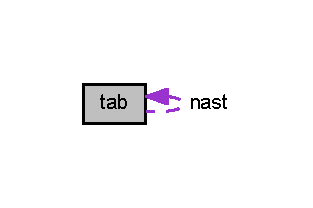
\includegraphics[width=150pt]{structtab__coll__graph}
\end{center}
\end{figure}
\subsection*{Atrybuty publiczne}
\begin{DoxyCompactItemize}
\item 
int $\ast$ \hyperlink{structtab_ad2b320d15f1496ed3147a7cdb2e5e1fb}{W}
\begin{DoxyCompactList}\small\item\em wskaźnik tablicy liczby wygranych gier \end{DoxyCompactList}\item 
int $\ast$ \hyperlink{structtab_acc9e4ee7e5e6df2449875e0a1dc67b18}{R}
\begin{DoxyCompactList}\small\item\em wskaźnik tablicy liczby zremisowanych gier \end{DoxyCompactList}\item 
int $\ast$ \hyperlink{structtab_aa99978b9e36e661312d4ac4581421a28}{P}
\begin{DoxyCompactList}\small\item\em wskaźnik tablicy liczby przegranych gier \end{DoxyCompactList}\item 
int \hyperlink{structtab_a8b52ff4e9a57646f4890690e1266c16f}{nruchu}
\begin{DoxyCompactList}\small\item\em numer kolejnego wykonywanego ruchu w drzewie / poziom drzewa \end{DoxyCompactList}\item 
\hyperlink{structtab}{tab} $\ast$ \hyperlink{structtab_abca0375dfae9e97ee6b0457d3b562ac9}{nast}
\begin{DoxyCompactList}\small\item\em wskaźnik na następny element listy \end{DoxyCompactList}\end{DoxyCompactItemize}


\subsection{Opis szczegółowy}
Element listy dynamicznej tablic. 

Definicja elementu dynamicznej lity tablic. Tablice zawierają liczbę wygranych, remisów i przegranych dla kopmutera dla jednego poziomu drzewa. 

\subsection{Dokumentacja atrybutów składowych}
\index{tab@{tab}!nast@{nast}}
\index{nast@{nast}!tab@{tab}}
\subsubsection[{\texorpdfstring{nast}{nast}}]{\setlength{\rightskip}{0pt plus 5cm}{\bf tab}$\ast$ tab\+::nast}\hypertarget{structtab_abca0375dfae9e97ee6b0457d3b562ac9}{}\label{structtab_abca0375dfae9e97ee6b0457d3b562ac9}


wskaźnik na następny element listy 

\index{tab@{tab}!nruchu@{nruchu}}
\index{nruchu@{nruchu}!tab@{tab}}
\subsubsection[{\texorpdfstring{nruchu}{nruchu}}]{\setlength{\rightskip}{0pt plus 5cm}int tab\+::nruchu}\hypertarget{structtab_a8b52ff4e9a57646f4890690e1266c16f}{}\label{structtab_a8b52ff4e9a57646f4890690e1266c16f}


numer kolejnego wykonywanego ruchu w drzewie / poziom drzewa 

\index{tab@{tab}!P@{P}}
\index{P@{P}!tab@{tab}}
\subsubsection[{\texorpdfstring{P}{P}}]{\setlength{\rightskip}{0pt plus 5cm}int$\ast$ tab\+::P}\hypertarget{structtab_aa99978b9e36e661312d4ac4581421a28}{}\label{structtab_aa99978b9e36e661312d4ac4581421a28}


wskaźnik tablicy liczby przegranych gier 

\index{tab@{tab}!R@{R}}
\index{R@{R}!tab@{tab}}
\subsubsection[{\texorpdfstring{R}{R}}]{\setlength{\rightskip}{0pt plus 5cm}int$\ast$ tab\+::R}\hypertarget{structtab_acc9e4ee7e5e6df2449875e0a1dc67b18}{}\label{structtab_acc9e4ee7e5e6df2449875e0a1dc67b18}


wskaźnik tablicy liczby zremisowanych gier 

\index{tab@{tab}!W@{W}}
\index{W@{W}!tab@{tab}}
\subsubsection[{\texorpdfstring{W}{W}}]{\setlength{\rightskip}{0pt plus 5cm}int$\ast$ tab\+::W}\hypertarget{structtab_ad2b320d15f1496ed3147a7cdb2e5e1fb}{}\label{structtab_ad2b320d15f1496ed3147a7cdb2e5e1fb}


wskaźnik tablicy liczby wygranych gier 



Dokumentacja dla tej struktury została wygenerowana z pliku\+:\begin{DoxyCompactItemize}
\item 
\hyperlink{tablice_8h}{tablice.\+h}\end{DoxyCompactItemize}

\hypertarget{structwezel}{}\section{Dokumentacja struktury wezel}
\label{structwezel}\index{wezel@{wezel}}


Element drzewa dynamicznego.  




{\ttfamily \#include $<$drzewo.\+h$>$}



Diagram współpracy dla wezel\+:\nopagebreak
\begin{figure}[H]
\begin{center}
\leavevmode
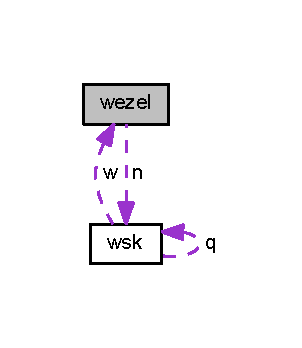
\includegraphics[width=145pt]{structwezel__coll__graph}
\end{center}
\end{figure}
\subsection*{Atrybuty publiczne}
\begin{DoxyCompactItemize}
\item 
char \hyperlink{structwezel_af8b190ce1c018baaf3d6b29c8b1703ca}{P} \mbox{[}3\mbox{]}\mbox{[}3\mbox{]}
\begin{DoxyCompactList}\small\item\em tablica -\/ plansza \end{DoxyCompactList}\item 
int \hyperlink{structwezel_a810cda81b39057158de9c45373bb6959}{nruchu}
\begin{DoxyCompactList}\small\item\em ilość możliwych do wykonania ruchów \end{DoxyCompactList}\item 
int \hyperlink{structwezel_ae0d7a5ffe5db5ae68d74ab8b796ef9d0}{gracz}
\begin{DoxyCompactList}\small\item\em znak danego gracza 1-\/\textquotesingle{}x\textquotesingle{} 2-\/\textquotesingle{}o\textquotesingle{} \end{DoxyCompactList}\item 
int \hyperlink{structwezel_aa2eeaaa4d77865a3a4d0e0fd4fbde30b}{nr}
\begin{DoxyCompactList}\small\item\em wykonywany ruch -\/ numer kolejnego możliwego ruchu \end{DoxyCompactList}\item 
int \hyperlink{structwezel_a87379e5872e2a13715421baec8dae5cf}{sytuacja}
\begin{DoxyCompactList}\small\item\em sytuacja na planszy 0-\/nieroztrzygnięta 1-\/wygrana komputera 2-\/wygrana gracza 3-\/remis \end{DoxyCompactList}\item 
struct \hyperlink{structwsk}{wsk} $\ast$ \hyperlink{structwezel_afa4e8d9b533246f9cf7d3ccdeefa2b3e}{n}
\begin{DoxyCompactList}\small\item\em wskaźnik na listę kolejnych elementów drzewa \end{DoxyCompactList}\end{DoxyCompactItemize}


\subsection{Opis szczegółowy}
Element drzewa dynamicznego. 

Definicja elementu dynamicznego drzewa możliwych ruchów. 

\subsection{Dokumentacja atrybutów składowych}
\index{wezel@{wezel}!gracz@{gracz}}
\index{gracz@{gracz}!wezel@{wezel}}
\subsubsection[{\texorpdfstring{gracz}{gracz}}]{\setlength{\rightskip}{0pt plus 5cm}int wezel\+::gracz}\hypertarget{structwezel_ae0d7a5ffe5db5ae68d74ab8b796ef9d0}{}\label{structwezel_ae0d7a5ffe5db5ae68d74ab8b796ef9d0}


znak danego gracza 1-\/\textquotesingle{}x\textquotesingle{} 2-\/\textquotesingle{}o\textquotesingle{} 

\index{wezel@{wezel}!n@{n}}
\index{n@{n}!wezel@{wezel}}
\subsubsection[{\texorpdfstring{n}{n}}]{\setlength{\rightskip}{0pt plus 5cm}struct {\bf wsk}$\ast$ wezel\+::n}\hypertarget{structwezel_afa4e8d9b533246f9cf7d3ccdeefa2b3e}{}\label{structwezel_afa4e8d9b533246f9cf7d3ccdeefa2b3e}


wskaźnik na listę kolejnych elementów drzewa 

\index{wezel@{wezel}!nr@{nr}}
\index{nr@{nr}!wezel@{wezel}}
\subsubsection[{\texorpdfstring{nr}{nr}}]{\setlength{\rightskip}{0pt plus 5cm}int wezel\+::nr}\hypertarget{structwezel_aa2eeaaa4d77865a3a4d0e0fd4fbde30b}{}\label{structwezel_aa2eeaaa4d77865a3a4d0e0fd4fbde30b}


wykonywany ruch -\/ numer kolejnego możliwego ruchu 

\index{wezel@{wezel}!nruchu@{nruchu}}
\index{nruchu@{nruchu}!wezel@{wezel}}
\subsubsection[{\texorpdfstring{nruchu}{nruchu}}]{\setlength{\rightskip}{0pt plus 5cm}int wezel\+::nruchu}\hypertarget{structwezel_a810cda81b39057158de9c45373bb6959}{}\label{structwezel_a810cda81b39057158de9c45373bb6959}


ilość możliwych do wykonania ruchów 

\index{wezel@{wezel}!P@{P}}
\index{P@{P}!wezel@{wezel}}
\subsubsection[{\texorpdfstring{P}{P}}]{\setlength{\rightskip}{0pt plus 5cm}char wezel\+::P\mbox{[}3\mbox{]}\mbox{[}3\mbox{]}}\hypertarget{structwezel_af8b190ce1c018baaf3d6b29c8b1703ca}{}\label{structwezel_af8b190ce1c018baaf3d6b29c8b1703ca}


tablica -\/ plansza 

\index{wezel@{wezel}!sytuacja@{sytuacja}}
\index{sytuacja@{sytuacja}!wezel@{wezel}}
\subsubsection[{\texorpdfstring{sytuacja}{sytuacja}}]{\setlength{\rightskip}{0pt plus 5cm}int wezel\+::sytuacja}\hypertarget{structwezel_a87379e5872e2a13715421baec8dae5cf}{}\label{structwezel_a87379e5872e2a13715421baec8dae5cf}


sytuacja na planszy 0-\/nieroztrzygnięta 1-\/wygrana komputera 2-\/wygrana gracza 3-\/remis 



Dokumentacja dla tej struktury została wygenerowana z pliku\+:\begin{DoxyCompactItemize}
\item 
\hyperlink{drzewo_8h}{drzewo.\+h}\end{DoxyCompactItemize}

\hypertarget{structwsk}{}\section{Dokumentacja struktury wsk}
\label{structwsk}\index{wsk@{wsk}}


Element listy w drzewie dynamicznym.  




{\ttfamily \#include $<$drzewo.\+h$>$}



Diagram współpracy dla wsk\+:\nopagebreak
\begin{figure}[H]
\begin{center}
\leavevmode
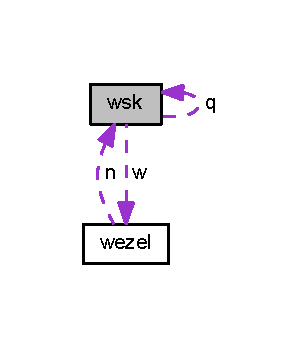
\includegraphics[width=145pt]{structwsk__coll__graph}
\end{center}
\end{figure}
\subsection*{Atrybuty publiczne}
\begin{DoxyCompactItemize}
\item 
\hyperlink{structwezel}{wezel} $\ast$ \hyperlink{structwsk_a69da68a1f76055e88538302c86ec7ac6}{w}
\begin{DoxyCompactList}\small\item\em wskaźnika na kolejny element drzewa \end{DoxyCompactList}\item 
\hyperlink{structwsk}{wsk} $\ast$ \hyperlink{structwsk_a5957f1d185b541d7572b8d9a11a8bf7d}{q}
\begin{DoxyCompactList}\small\item\em wskaźnik na kolejny element listy \end{DoxyCompactList}\end{DoxyCompactItemize}


\subsection{Opis szczegółowy}
Element listy w drzewie dynamicznym. 

Definicja elementu listy dynamicznej w drzewie. 

\subsection{Dokumentacja atrybutów składowych}
\index{wsk@{wsk}!q@{q}}
\index{q@{q}!wsk@{wsk}}
\subsubsection[{\texorpdfstring{q}{q}}]{\setlength{\rightskip}{0pt plus 5cm}{\bf wsk}$\ast$ wsk\+::q}\hypertarget{structwsk_a5957f1d185b541d7572b8d9a11a8bf7d}{}\label{structwsk_a5957f1d185b541d7572b8d9a11a8bf7d}


wskaźnik na kolejny element listy 

\index{wsk@{wsk}!w@{w}}
\index{w@{w}!wsk@{wsk}}
\subsubsection[{\texorpdfstring{w}{w}}]{\setlength{\rightskip}{0pt plus 5cm}{\bf wezel}$\ast$ wsk\+::w}\hypertarget{structwsk_a69da68a1f76055e88538302c86ec7ac6}{}\label{structwsk_a69da68a1f76055e88538302c86ec7ac6}


wskaźnika na kolejny element drzewa 



Dokumentacja dla tej struktury została wygenerowana z pliku\+:\begin{DoxyCompactItemize}
\item 
\hyperlink{drzewo_8h}{drzewo.\+h}\end{DoxyCompactItemize}

\chapter{Dokumentacja plików}
\hypertarget{drzewo_8cpp}{}\section{Dokumentacja pliku drzewo.\+cpp}
\label{drzewo_8cpp}\index{drzewo.\+cpp@{drzewo.\+cpp}}


Plik źródłowy modułu drzewo.  


{\ttfamily \#include \char`\"{}drzewo.\+h\char`\"{}}\\*
Wykres zależności załączania dla drzewo.\+cpp\+:\nopagebreak
\begin{figure}[H]
\begin{center}
\leavevmode
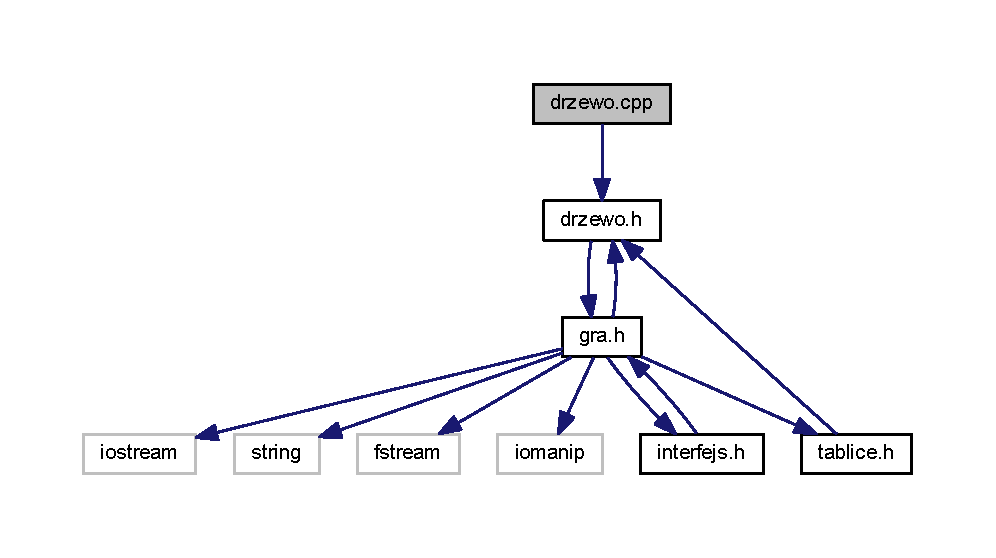
\includegraphics[width=350pt]{drzewo_8cpp__incl}
\end{center}
\end{figure}
\subsection*{Funkcje}
\begin{DoxyCompactItemize}
\item 
void \hyperlink{drzewo_8cpp_a8d34288192893c796076ba13c759685a}{t\+\_\+drzewo} (\hyperlink{structwezel}{wezel} $\ast$pop, int poziom, char znakk)
\begin{DoxyCompactList}\small\item\em Rekurencyjne tworzenie drzewa. \end{DoxyCompactList}\item 
void \hyperlink{drzewo_8cpp_a1dbe44033e123ea16882bb48f91b9bc3}{usun\+\_\+bok} (\hyperlink{structwsk}{wsk} $\ast$\&n)
\begin{DoxyCompactList}\small\item\em Usuwanie listy w drzewie. \end{DoxyCompactList}\item 
void \hyperlink{drzewo_8cpp_ad4d63b25f7d0462a217e05cf2da8849f}{usun\+\_\+drzewo} (\hyperlink{structwezel}{wezel} $\ast$\&kor)
\begin{DoxyCompactList}\small\item\em Usuwanie drzewa. \end{DoxyCompactList}\item 
\hyperlink{structwezel}{wezel} $\ast$ \hyperlink{drzewo_8cpp_a90322c22721610cd4c5a812fcdd0427c}{drzewo} (char T\mbox{[}3\mbox{]}\mbox{[}3\mbox{]}, char znakk)
\begin{DoxyCompactList}\small\item\em Nowe drzewo. \end{DoxyCompactList}\item 
void \hyperlink{drzewo_8cpp_aee17db8f1899626ab6f4ca2b010d3569}{przepisz} (char T\mbox{[}3\mbox{]}\mbox{[}3\mbox{]}, char P\mbox{[}3\mbox{]}\mbox{[}3\mbox{]})
\begin{DoxyCompactList}\small\item\em Przepisywanie tablicy. \end{DoxyCompactList}\item 
void \hyperlink{drzewo_8cpp_a025cadf1c2c5401689aa77bc194057a5}{lepsze} (\hyperlink{structwezel}{wezel} $\ast$pop)
\begin{DoxyCompactList}\small\item\em Ulepszenie drzewa. \end{DoxyCompactList}\item 
void \hyperlink{drzewo_8cpp_a029b2288db51eebfd1282e2f9323086c}{sprawdz\+\_\+poziom} (\hyperlink{structwezel}{wezel} $\ast$pop)
\begin{DoxyCompactList}\small\item\em Usuwanie ruchów. \end{DoxyCompactList}\end{DoxyCompactItemize}


\subsection{Opis szczegółowy}
Plik źródłowy modułu drzewo. 



\subsection{Dokumentacja funkcji}
\index{drzewo.\+cpp@{drzewo.\+cpp}!drzewo@{drzewo}}
\index{drzewo@{drzewo}!drzewo.\+cpp@{drzewo.\+cpp}}
\subsubsection[{\texorpdfstring{drzewo(char T[3][3], char znakk)}{drzewo(char T[3][3], char znakk)}}]{\setlength{\rightskip}{0pt plus 5cm}{\bf wezel}$\ast$ drzewo (
\begin{DoxyParamCaption}
\item[{char}]{T\mbox{[}3\mbox{]}\mbox{[}3\mbox{]}, }
\item[{char}]{znakk}
\end{DoxyParamCaption}
)}\hypertarget{drzewo_8cpp_a90322c22721610cd4c5a812fcdd0427c}{}\label{drzewo_8cpp_a90322c22721610cd4c5a812fcdd0427c}


Nowe drzewo. 

Funkcja tworząca nowe drzewo wszystkich możliwych ruchów. 
\begin{DoxyParams}{Parametry}
{\em T} & aktualna plansza \\
\hline
{\em znakk} & znak którym gra komputer \\
\hline
\end{DoxyParams}
\begin{DoxyReturn}{Zwraca}
korzeń nowego drzewa 
\end{DoxyReturn}
\index{drzewo.\+cpp@{drzewo.\+cpp}!lepsze@{lepsze}}
\index{lepsze@{lepsze}!drzewo.\+cpp@{drzewo.\+cpp}}
\subsubsection[{\texorpdfstring{lepsze(wezel $\ast$pop)}{lepsze(wezel *pop)}}]{\setlength{\rightskip}{0pt plus 5cm}void lepsze (
\begin{DoxyParamCaption}
\item[{{\bf wezel} $\ast$}]{pop}
\end{DoxyParamCaption}
)}\hypertarget{drzewo_8cpp_a025cadf1c2c5401689aa77bc194057a5}{}\label{drzewo_8cpp_a025cadf1c2c5401689aa77bc194057a5}


Ulepszenie drzewa. 

Procedura usuwająca inne ruchy możliwe dla gracza jeżeli ma możilwy ruch wygrywający. Procedura rekurencyjna. 
\begin{DoxyParams}{Parametry}
{\em pop} & poprzedni element drzewa w funkcji rejkurencyjnej \\
\hline
\end{DoxyParams}
\index{drzewo.\+cpp@{drzewo.\+cpp}!przepisz@{przepisz}}
\index{przepisz@{przepisz}!drzewo.\+cpp@{drzewo.\+cpp}}
\subsubsection[{\texorpdfstring{przepisz(char T[3][3], char P[3][3])}{przepisz(char T[3][3], char P[3][3])}}]{\setlength{\rightskip}{0pt plus 5cm}void przepisz (
\begin{DoxyParamCaption}
\item[{char}]{T\mbox{[}3\mbox{]}\mbox{[}3\mbox{]}, }
\item[{char}]{P\mbox{[}3\mbox{]}\mbox{[}3\mbox{]}}
\end{DoxyParamCaption}
)}\hypertarget{drzewo_8cpp_aee17db8f1899626ab6f4ca2b010d3569}{}\label{drzewo_8cpp_aee17db8f1899626ab6f4ca2b010d3569}


Przepisywanie tablicy. 

Procedura przepisująca elementy z jednej tablicy do drugiej. 
\begin{DoxyParams}{Parametry}
{\em T} & tablica do której przepisujemy elementy \\
\hline
{\em P} & tablica z której przepisujemy elementy \\
\hline
\end{DoxyParams}
\index{drzewo.\+cpp@{drzewo.\+cpp}!sprawdz\+\_\+poziom@{sprawdz\+\_\+poziom}}
\index{sprawdz\+\_\+poziom@{sprawdz\+\_\+poziom}!drzewo.\+cpp@{drzewo.\+cpp}}
\subsubsection[{\texorpdfstring{sprawdz\+\_\+poziom(wezel $\ast$pop)}{sprawdz_poziom(wezel *pop)}}]{\setlength{\rightskip}{0pt plus 5cm}void sprawdz\+\_\+poziom (
\begin{DoxyParamCaption}
\item[{{\bf wezel} $\ast$}]{pop}
\end{DoxyParamCaption}
)}\hypertarget{drzewo_8cpp_a029b2288db51eebfd1282e2f9323086c}{}\label{drzewo_8cpp_a029b2288db51eebfd1282e2f9323086c}


Usuwanie ruchów. 

Procedura usuwająca inne możliwe ruchy gracza, gdy istnieje jego ruch wygrywający w danym poziomie drzewa. 
\begin{DoxyParams}{Parametry}
{\em pop} & element drzewa \\
\hline
\end{DoxyParams}
\index{drzewo.\+cpp@{drzewo.\+cpp}!t\+\_\+drzewo@{t\+\_\+drzewo}}
\index{t\+\_\+drzewo@{t\+\_\+drzewo}!drzewo.\+cpp@{drzewo.\+cpp}}
\subsubsection[{\texorpdfstring{t\+\_\+drzewo(wezel $\ast$pop, int poziom, char znakk)}{t_drzewo(wezel *pop, int poziom, char znakk)}}]{\setlength{\rightskip}{0pt plus 5cm}void t\+\_\+drzewo (
\begin{DoxyParamCaption}
\item[{{\bf wezel} $\ast$}]{pop, }
\item[{int}]{poziom, }
\item[{char}]{znakk}
\end{DoxyParamCaption}
)}\hypertarget{drzewo_8cpp_a8d34288192893c796076ba13c759685a}{}\label{drzewo_8cpp_a8d34288192893c796076ba13c759685a}


Rekurencyjne tworzenie drzewa. 

Procedura rekurencyjna do tworzenia drzewa. 
\begin{DoxyParams}{Parametry}
{\em pop} & wskaźnik poprzedniego elementu \\
\hline
{\em poziom} & ilość początkowych możliwych ruchów \\
\hline
{\em znakk} & znak którym gra komputer \\
\hline
\end{DoxyParams}
\index{drzewo.\+cpp@{drzewo.\+cpp}!usun\+\_\+bok@{usun\+\_\+bok}}
\index{usun\+\_\+bok@{usun\+\_\+bok}!drzewo.\+cpp@{drzewo.\+cpp}}
\subsubsection[{\texorpdfstring{usun\+\_\+bok(wsk $\ast$\&n)}{usun_bok(wsk *&n)}}]{\setlength{\rightskip}{0pt plus 5cm}void usun\+\_\+bok (
\begin{DoxyParamCaption}
\item[{{\bf wsk} $\ast$\&}]{n}
\end{DoxyParamCaption}
)}\hypertarget{drzewo_8cpp_a1dbe44033e123ea16882bb48f91b9bc3}{}\label{drzewo_8cpp_a1dbe44033e123ea16882bb48f91b9bc3}


Usuwanie listy w drzewie. 

Procedura pomocnicza przy usuwaniu drzewa, usuwająca listy dynamiczne zawarte w drzewie. 
\begin{DoxyParams}{Parametry}
{\em n} & wskaźnik na pierwszy element listy \\
\hline
\end{DoxyParams}
\index{drzewo.\+cpp@{drzewo.\+cpp}!usun\+\_\+drzewo@{usun\+\_\+drzewo}}
\index{usun\+\_\+drzewo@{usun\+\_\+drzewo}!drzewo.\+cpp@{drzewo.\+cpp}}
\subsubsection[{\texorpdfstring{usun\+\_\+drzewo(wezel $\ast$\&kor)}{usun_drzewo(wezel *&kor)}}]{\setlength{\rightskip}{0pt plus 5cm}void usun\+\_\+drzewo (
\begin{DoxyParamCaption}
\item[{{\bf wezel} $\ast$\&}]{kor}
\end{DoxyParamCaption}
)}\hypertarget{drzewo_8cpp_ad4d63b25f7d0462a217e05cf2da8849f}{}\label{drzewo_8cpp_ad4d63b25f7d0462a217e05cf2da8849f}


Usuwanie drzewa. 

Procedura usuwająca drzewo. 
\begin{DoxyParams}{Parametry}
{\em kor} & korzeń drzewa \\
\hline
\end{DoxyParams}

\hypertarget{drzewo_8h}{}\section{Dokumentacja pliku drzewo.\+h}
\label{drzewo_8h}\index{drzewo.\+h@{drzewo.\+h}}


Plik nagłówkowy modułu drzewo.  


{\ttfamily \#include \char`\"{}gra.\+h\char`\"{}}\\*
Wykres zależności załączania dla drzewo.\+h\+:\nopagebreak
\begin{figure}[H]
\begin{center}
\leavevmode
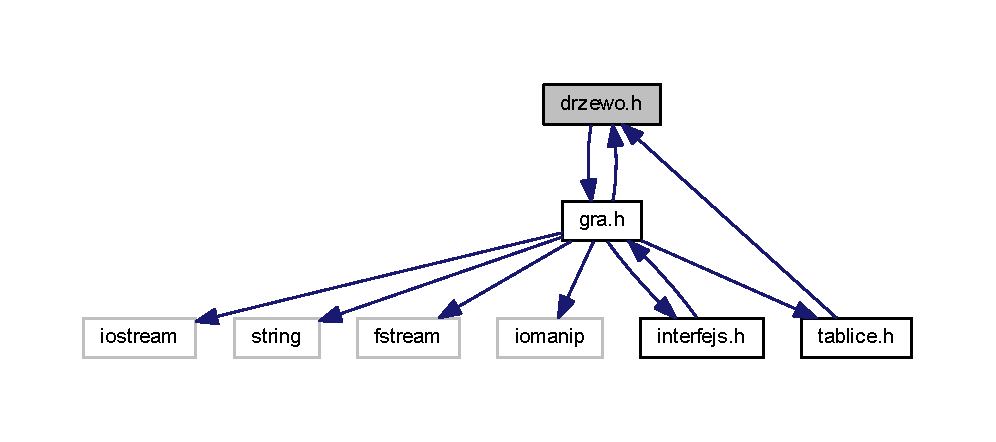
\includegraphics[width=350pt]{drzewo_8h__incl}
\end{center}
\end{figure}
Ten wykres pokazuje, które pliki bezpośrednio lub pośrednio załączają ten plik\+:\nopagebreak
\begin{figure}[H]
\begin{center}
\leavevmode
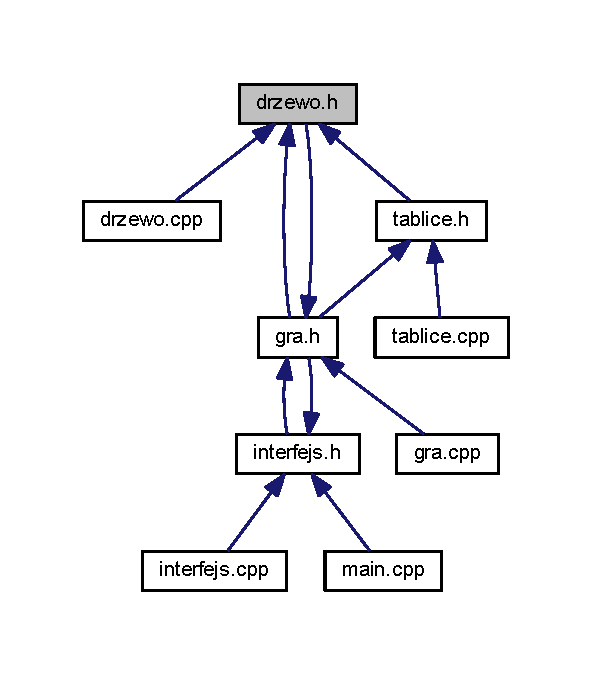
\includegraphics[width=284pt]{drzewo_8h__dep__incl}
\end{center}
\end{figure}
\subsection*{Komponenty}
\begin{DoxyCompactItemize}
\item 
struct \hyperlink{structwezel}{wezel}
\begin{DoxyCompactList}\small\item\em Element drzewa dynamicznego. \end{DoxyCompactList}\item 
struct \hyperlink{structwsk}{wsk}
\begin{DoxyCompactList}\small\item\em Element listy w drzewie dynamicznym. \end{DoxyCompactList}\end{DoxyCompactItemize}
\subsection*{Funkcje}
\begin{DoxyCompactItemize}
\item 
\hyperlink{structwezel}{wezel} $\ast$ \hyperlink{drzewo_8h_a90322c22721610cd4c5a812fcdd0427c}{drzewo} (char T\mbox{[}3\mbox{]}\mbox{[}3\mbox{]}, char znakk)
\begin{DoxyCompactList}\small\item\em Nowe drzewo. \end{DoxyCompactList}\item 
void \hyperlink{drzewo_8h_ad4d63b25f7d0462a217e05cf2da8849f}{usun\+\_\+drzewo} (\hyperlink{structwezel}{wezel} $\ast$\&kor)
\begin{DoxyCompactList}\small\item\em Usuwanie drzewa. \end{DoxyCompactList}\item 
void \hyperlink{drzewo_8h_a1dbe44033e123ea16882bb48f91b9bc3}{usun\+\_\+bok} (\hyperlink{structwsk}{wsk} $\ast$\&n)
\begin{DoxyCompactList}\small\item\em Usuwanie listy w drzewie. \end{DoxyCompactList}\item 
void \hyperlink{drzewo_8h_a8d34288192893c796076ba13c759685a}{t\+\_\+drzewo} (\hyperlink{structwezel}{wezel} $\ast$pop, int poziom, char znakk)
\begin{DoxyCompactList}\small\item\em Rekurencyjne tworzenie drzewa. \end{DoxyCompactList}\item 
void \hyperlink{drzewo_8h_aee17db8f1899626ab6f4ca2b010d3569}{przepisz} (char T\mbox{[}3\mbox{]}\mbox{[}3\mbox{]}, char P\mbox{[}3\mbox{]}\mbox{[}3\mbox{]})
\begin{DoxyCompactList}\small\item\em Przepisywanie tablicy. \end{DoxyCompactList}\item 
void \hyperlink{drzewo_8h_a025cadf1c2c5401689aa77bc194057a5}{lepsze} (\hyperlink{structwezel}{wezel} $\ast$pop)
\begin{DoxyCompactList}\small\item\em Ulepszenie drzewa. \end{DoxyCompactList}\item 
void \hyperlink{drzewo_8h_a029b2288db51eebfd1282e2f9323086c}{sprawdz\+\_\+poziom} (\hyperlink{structwezel}{wezel} $\ast$pop)
\begin{DoxyCompactList}\small\item\em Usuwanie ruchów. \end{DoxyCompactList}\end{DoxyCompactItemize}


\subsection{Opis szczegółowy}
Plik nagłówkowy modułu drzewo. 



\subsection{Dokumentacja funkcji}
\index{drzewo.\+h@{drzewo.\+h}!drzewo@{drzewo}}
\index{drzewo@{drzewo}!drzewo.\+h@{drzewo.\+h}}
\subsubsection[{\texorpdfstring{drzewo(char T[3][3], char znakk)}{drzewo(char T[3][3], char znakk)}}]{\setlength{\rightskip}{0pt plus 5cm}{\bf wezel}$\ast$ drzewo (
\begin{DoxyParamCaption}
\item[{char}]{T\mbox{[}3\mbox{]}\mbox{[}3\mbox{]}, }
\item[{char}]{znakk}
\end{DoxyParamCaption}
)}\hypertarget{drzewo_8h_a90322c22721610cd4c5a812fcdd0427c}{}\label{drzewo_8h_a90322c22721610cd4c5a812fcdd0427c}


Nowe drzewo. 

Funkcja tworząca nowe drzewo wszystkich możliwych ruchów. 
\begin{DoxyParams}{Parametry}
{\em T} & aktualna plansza \\
\hline
{\em znakk} & znak którym gra komputer \\
\hline
\end{DoxyParams}
\begin{DoxyReturn}{Zwraca}
korzeń nowego drzewa 
\end{DoxyReturn}
\index{drzewo.\+h@{drzewo.\+h}!lepsze@{lepsze}}
\index{lepsze@{lepsze}!drzewo.\+h@{drzewo.\+h}}
\subsubsection[{\texorpdfstring{lepsze(wezel $\ast$pop)}{lepsze(wezel *pop)}}]{\setlength{\rightskip}{0pt plus 5cm}void lepsze (
\begin{DoxyParamCaption}
\item[{{\bf wezel} $\ast$}]{pop}
\end{DoxyParamCaption}
)}\hypertarget{drzewo_8h_a025cadf1c2c5401689aa77bc194057a5}{}\label{drzewo_8h_a025cadf1c2c5401689aa77bc194057a5}


Ulepszenie drzewa. 

Procedura usuwająca inne ruchy możliwe dla gracza jeżeli ma możilwy ruch wygrywający. Procedura rekurencyjna. 
\begin{DoxyParams}{Parametry}
{\em pop} & poprzedni element drzewa w funkcji rejkurencyjnej \\
\hline
\end{DoxyParams}
\index{drzewo.\+h@{drzewo.\+h}!przepisz@{przepisz}}
\index{przepisz@{przepisz}!drzewo.\+h@{drzewo.\+h}}
\subsubsection[{\texorpdfstring{przepisz(char T[3][3], char P[3][3])}{przepisz(char T[3][3], char P[3][3])}}]{\setlength{\rightskip}{0pt plus 5cm}void przepisz (
\begin{DoxyParamCaption}
\item[{char}]{T\mbox{[}3\mbox{]}\mbox{[}3\mbox{]}, }
\item[{char}]{P\mbox{[}3\mbox{]}\mbox{[}3\mbox{]}}
\end{DoxyParamCaption}
)}\hypertarget{drzewo_8h_aee17db8f1899626ab6f4ca2b010d3569}{}\label{drzewo_8h_aee17db8f1899626ab6f4ca2b010d3569}


Przepisywanie tablicy. 

Procedura przepisująca elementy z jednej tablicy do drugiej. 
\begin{DoxyParams}{Parametry}
{\em T} & tablica do której przepisujemy elementy \\
\hline
{\em P} & tablica z której przepisujemy elementy \\
\hline
\end{DoxyParams}
\index{drzewo.\+h@{drzewo.\+h}!sprawdz\+\_\+poziom@{sprawdz\+\_\+poziom}}
\index{sprawdz\+\_\+poziom@{sprawdz\+\_\+poziom}!drzewo.\+h@{drzewo.\+h}}
\subsubsection[{\texorpdfstring{sprawdz\+\_\+poziom(wezel $\ast$pop)}{sprawdz_poziom(wezel *pop)}}]{\setlength{\rightskip}{0pt plus 5cm}void sprawdz\+\_\+poziom (
\begin{DoxyParamCaption}
\item[{{\bf wezel} $\ast$}]{pop}
\end{DoxyParamCaption}
)}\hypertarget{drzewo_8h_a029b2288db51eebfd1282e2f9323086c}{}\label{drzewo_8h_a029b2288db51eebfd1282e2f9323086c}


Usuwanie ruchów. 

Procedura usuwająca inne możliwe ruchy gracza, gdy istnieje jego ruch wygrywający w danym poziomie drzewa. 
\begin{DoxyParams}{Parametry}
{\em pop} & element drzewa \\
\hline
\end{DoxyParams}
\index{drzewo.\+h@{drzewo.\+h}!t\+\_\+drzewo@{t\+\_\+drzewo}}
\index{t\+\_\+drzewo@{t\+\_\+drzewo}!drzewo.\+h@{drzewo.\+h}}
\subsubsection[{\texorpdfstring{t\+\_\+drzewo(wezel $\ast$pop, int poziom, char znakk)}{t_drzewo(wezel *pop, int poziom, char znakk)}}]{\setlength{\rightskip}{0pt plus 5cm}void t\+\_\+drzewo (
\begin{DoxyParamCaption}
\item[{{\bf wezel} $\ast$}]{pop, }
\item[{int}]{poziom, }
\item[{char}]{znakk}
\end{DoxyParamCaption}
)}\hypertarget{drzewo_8h_a8d34288192893c796076ba13c759685a}{}\label{drzewo_8h_a8d34288192893c796076ba13c759685a}


Rekurencyjne tworzenie drzewa. 

Procedura rekurencyjna do tworzenia drzewa. 
\begin{DoxyParams}{Parametry}
{\em pop} & wskaźnik poprzedniego elementu \\
\hline
{\em poziom} & ilość początkowych możliwych ruchów \\
\hline
{\em znakk} & znak którym gra komputer \\
\hline
\end{DoxyParams}
\index{drzewo.\+h@{drzewo.\+h}!usun\+\_\+bok@{usun\+\_\+bok}}
\index{usun\+\_\+bok@{usun\+\_\+bok}!drzewo.\+h@{drzewo.\+h}}
\subsubsection[{\texorpdfstring{usun\+\_\+bok(wsk $\ast$\&n)}{usun_bok(wsk *&n)}}]{\setlength{\rightskip}{0pt plus 5cm}void usun\+\_\+bok (
\begin{DoxyParamCaption}
\item[{{\bf wsk} $\ast$\&}]{n}
\end{DoxyParamCaption}
)}\hypertarget{drzewo_8h_a1dbe44033e123ea16882bb48f91b9bc3}{}\label{drzewo_8h_a1dbe44033e123ea16882bb48f91b9bc3}


Usuwanie listy w drzewie. 

Procedura pomocnicza przy usuwaniu drzewa, usuwająca listy dynamiczne zawarte w drzewie. 
\begin{DoxyParams}{Parametry}
{\em n} & wskaźnik na pierwszy element listy \\
\hline
\end{DoxyParams}
\index{drzewo.\+h@{drzewo.\+h}!usun\+\_\+drzewo@{usun\+\_\+drzewo}}
\index{usun\+\_\+drzewo@{usun\+\_\+drzewo}!drzewo.\+h@{drzewo.\+h}}
\subsubsection[{\texorpdfstring{usun\+\_\+drzewo(wezel $\ast$\&kor)}{usun_drzewo(wezel *&kor)}}]{\setlength{\rightskip}{0pt plus 5cm}void usun\+\_\+drzewo (
\begin{DoxyParamCaption}
\item[{{\bf wezel} $\ast$\&}]{kor}
\end{DoxyParamCaption}
)}\hypertarget{drzewo_8h_ad4d63b25f7d0462a217e05cf2da8849f}{}\label{drzewo_8h_ad4d63b25f7d0462a217e05cf2da8849f}


Usuwanie drzewa. 

Procedura usuwająca drzewo. 
\begin{DoxyParams}{Parametry}
{\em kor} & korzeń drzewa \\
\hline
\end{DoxyParams}

\hypertarget{gra_8cpp}{}\section{Dokumentacja pliku gra.\+cpp}
\label{gra_8cpp}\index{gra.\+cpp@{gra.\+cpp}}


Plik źródłowy modułu gra.  


{\ttfamily \#include \char`\"{}gra.\+h\char`\"{}}\\*
Wykres zależności załączania dla gra.\+cpp\+:\nopagebreak
\begin{figure}[H]
\begin{center}
\leavevmode
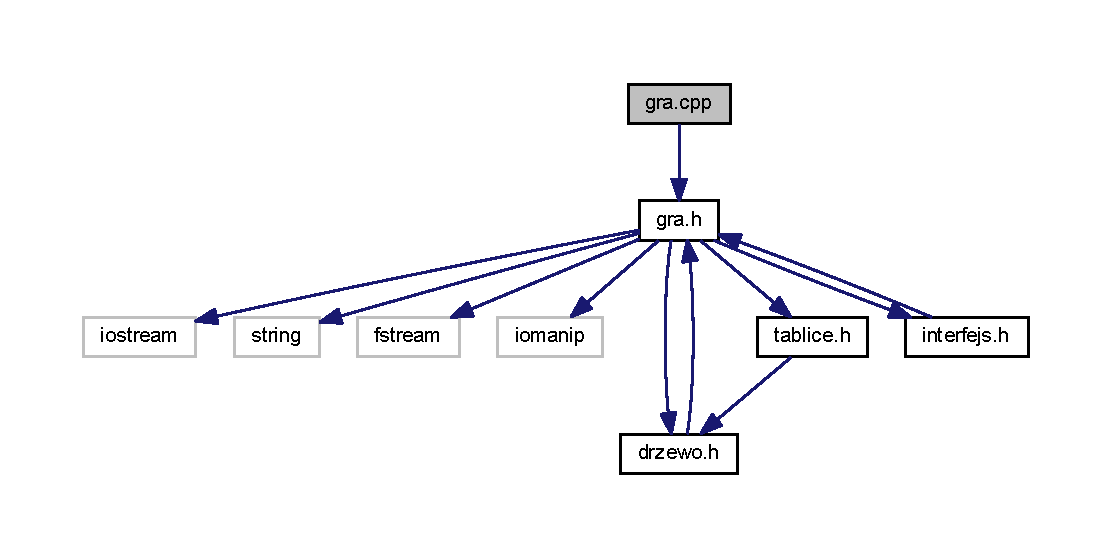
\includegraphics[width=350pt]{gra_8cpp__incl}
\end{center}
\end{figure}
\subsection*{Funkcje}
\begin{DoxyCompactItemize}
\item 
void \hyperlink{gra_8cpp_ab0797c12c305cbec795147e947ec1e39}{nowa\+\_\+plansza} (char T\mbox{[}3\mbox{]}\mbox{[}3\mbox{]})
\begin{DoxyCompactList}\small\item\em Nowa plansza. \end{DoxyCompactList}\item 
void \hyperlink{gra_8cpp_ac74b2e179aafb0d5ace62ae1912cdb70}{wpisz\+\_\+tab} (char T\mbox{[}3\mbox{]}\mbox{[}3\mbox{]}, int n, char znak)
\begin{DoxyCompactList}\small\item\em Wpisywanie ruchu do planszy. \end{DoxyCompactList}\item 
int \hyperlink{gra_8cpp_a23182285f4fd1e760bdf5d29101488a1}{wygrana} (char T\mbox{[}3\mbox{]}\mbox{[}3\mbox{]})
\begin{DoxyCompactList}\small\item\em Sprawdzanie sytuacji. \end{DoxyCompactList}\item 
void \hyperlink{gra_8cpp_a472d54e5297c6dfea59903654de33ee8}{gra} ()
\begin{DoxyCompactList}\small\item\em Gra. \end{DoxyCompactList}\item 
void \hyperlink{gra_8cpp_ae9feff07994880d9f0164bbad6aff388}{wpisz\+\_\+do\+\_\+wyniki} (int l, string nowe)
\begin{DoxyCompactList}\small\item\em Wpisywanie do wyników. \end{DoxyCompactList}\end{DoxyCompactItemize}


\subsection{Opis szczegółowy}
Plik źródłowy modułu gra. 



\subsection{Dokumentacja funkcji}
\index{gra.\+cpp@{gra.\+cpp}!gra@{gra}}
\index{gra@{gra}!gra.\+cpp@{gra.\+cpp}}
\subsubsection[{\texorpdfstring{gra()}{gra()}}]{\setlength{\rightskip}{0pt plus 5cm}void gra (
\begin{DoxyParamCaption}
{}
\end{DoxyParamCaption}
)}\hypertarget{gra_8cpp_a472d54e5297c6dfea59903654de33ee8}{}\label{gra_8cpp_a472d54e5297c6dfea59903654de33ee8}


Gra. 

Procedura przeprowadzająca grę. \index{gra.\+cpp@{gra.\+cpp}!nowa\+\_\+plansza@{nowa\+\_\+plansza}}
\index{nowa\+\_\+plansza@{nowa\+\_\+plansza}!gra.\+cpp@{gra.\+cpp}}
\subsubsection[{\texorpdfstring{nowa\+\_\+plansza(char T[3][3])}{nowa_plansza(char T[3][3])}}]{\setlength{\rightskip}{0pt plus 5cm}void nowa\+\_\+plansza (
\begin{DoxyParamCaption}
\item[{char}]{T\mbox{[}3\mbox{]}\mbox{[}3\mbox{]}}
\end{DoxyParamCaption}
)}\hypertarget{gra_8cpp_ab0797c12c305cbec795147e947ec1e39}{}\label{gra_8cpp_ab0797c12c305cbec795147e947ec1e39}


Nowa plansza. 

Procedura wypełniająca planszę znakami \textquotesingle{}-\/\textquotesingle{}. 
\begin{DoxyParams}{Parametry}
{\em T} & plansza \\
\hline
\end{DoxyParams}
\index{gra.\+cpp@{gra.\+cpp}!wpisz\+\_\+do\+\_\+wyniki@{wpisz\+\_\+do\+\_\+wyniki}}
\index{wpisz\+\_\+do\+\_\+wyniki@{wpisz\+\_\+do\+\_\+wyniki}!gra.\+cpp@{gra.\+cpp}}
\subsubsection[{\texorpdfstring{wpisz\+\_\+do\+\_\+wyniki(int l, string nowe)}{wpisz_do_wyniki(int l, string nowe)}}]{\setlength{\rightskip}{0pt plus 5cm}void wpisz\+\_\+do\+\_\+wyniki (
\begin{DoxyParamCaption}
\item[{int}]{l, }
\item[{string}]{nowe}
\end{DoxyParamCaption}
)}\hypertarget{gra_8cpp_ae9feff07994880d9f0164bbad6aff388}{}\label{gra_8cpp_ae9feff07994880d9f0164bbad6aff388}


Wpisywanie do wyników. 

Procedura dopisująca wyniku do pliku \char`\"{}wyniki.\+txt\char`\"{}. 
\begin{DoxyParams}{Parametry}
{\em l} & parametr mówiący czy dopisać wygraną(l=1), czy remis(l=0). \\
\hline
{\em nowe} & nowa nazwa gracza \\
\hline
\end{DoxyParams}
\index{gra.\+cpp@{gra.\+cpp}!wpisz\+\_\+tab@{wpisz\+\_\+tab}}
\index{wpisz\+\_\+tab@{wpisz\+\_\+tab}!gra.\+cpp@{gra.\+cpp}}
\subsubsection[{\texorpdfstring{wpisz\+\_\+tab(char T[3][3], int n, char znak)}{wpisz_tab(char T[3][3], int n, char znak)}}]{\setlength{\rightskip}{0pt plus 5cm}void wpisz\+\_\+tab (
\begin{DoxyParamCaption}
\item[{char}]{T\mbox{[}3\mbox{]}\mbox{[}3\mbox{]}, }
\item[{int}]{n, }
\item[{char}]{znak}
\end{DoxyParamCaption}
)}\hypertarget{gra_8cpp_ac74b2e179aafb0d5ace62ae1912cdb70}{}\label{gra_8cpp_ac74b2e179aafb0d5ace62ae1912cdb70}


Wpisywanie ruchu do planszy. 

Procedura wpisująca dany znak do n-\/tego wolnego miejsca na planszy T. 
\begin{DoxyParams}{Parametry}
{\em T} & plansza \\
\hline
{\em n} & numer ruchu \\
\hline
{\em znak} & znak do wpisania \\
\hline
\end{DoxyParams}
\index{gra.\+cpp@{gra.\+cpp}!wygrana@{wygrana}}
\index{wygrana@{wygrana}!gra.\+cpp@{gra.\+cpp}}
\subsubsection[{\texorpdfstring{wygrana(char T[3][3])}{wygrana(char T[3][3])}}]{\setlength{\rightskip}{0pt plus 5cm}int wygrana (
\begin{DoxyParamCaption}
\item[{char}]{T\mbox{[}3\mbox{]}\mbox{[}3\mbox{]}}
\end{DoxyParamCaption}
)}\hypertarget{gra_8cpp_a23182285f4fd1e760bdf5d29101488a1}{}\label{gra_8cpp_a23182285f4fd1e760bdf5d29101488a1}


Sprawdzanie sytuacji. 

Funkcja zwracająca w jakiej sytuacji znajduje się plansza. Zwraca 0-\/nieroztrzygnięta 1-\/wygrana kółka 2-\/wygrana krzyżyka 3-\/remis 
\begin{DoxyParams}{Parametry}
{\em T} & plansza \\
\hline
\end{DoxyParams}
\begin{DoxyReturn}{Zwraca}
sytuacja 
\end{DoxyReturn}

\hypertarget{gra_8h}{}\section{Dokumentacja pliku gra.\+h}
\label{gra_8h}\index{gra.\+h@{gra.\+h}}


Plik nagłówkowy modułu gra.  


{\ttfamily \#include $<$iostream$>$}\\*
{\ttfamily \#include $<$string$>$}\\*
{\ttfamily \#include $<$fstream$>$}\\*
{\ttfamily \#include $<$iomanip$>$}\\*
{\ttfamily \#include \char`\"{}drzewo.\+h\char`\"{}}\\*
{\ttfamily \#include \char`\"{}tablice.\+h\char`\"{}}\\*
{\ttfamily \#include \char`\"{}interfejs.\+h\char`\"{}}\\*
Wykres zależności załączania dla gra.\+h\+:\nopagebreak
\begin{figure}[H]
\begin{center}
\leavevmode
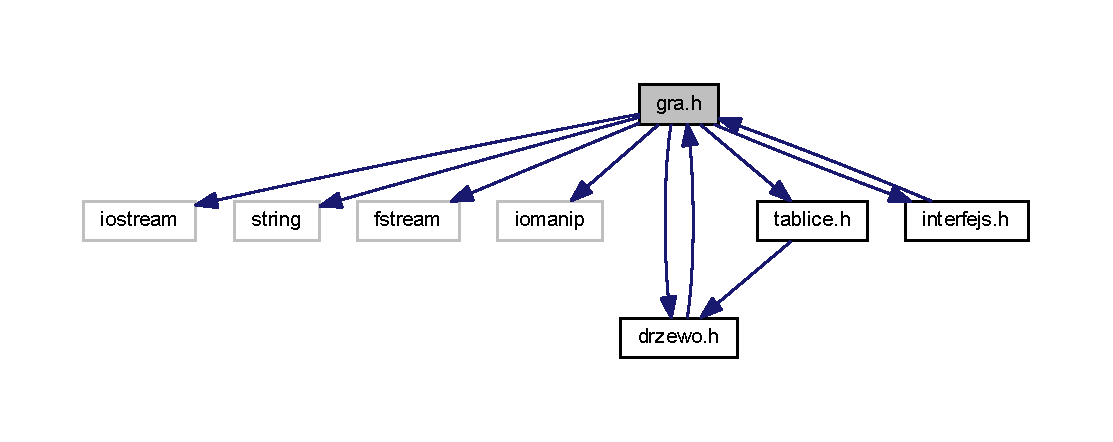
\includegraphics[width=350pt]{gra_8h__incl}
\end{center}
\end{figure}
Ten wykres pokazuje, które pliki bezpośrednio lub pośrednio załączają ten plik\+:\nopagebreak
\begin{figure}[H]
\begin{center}
\leavevmode
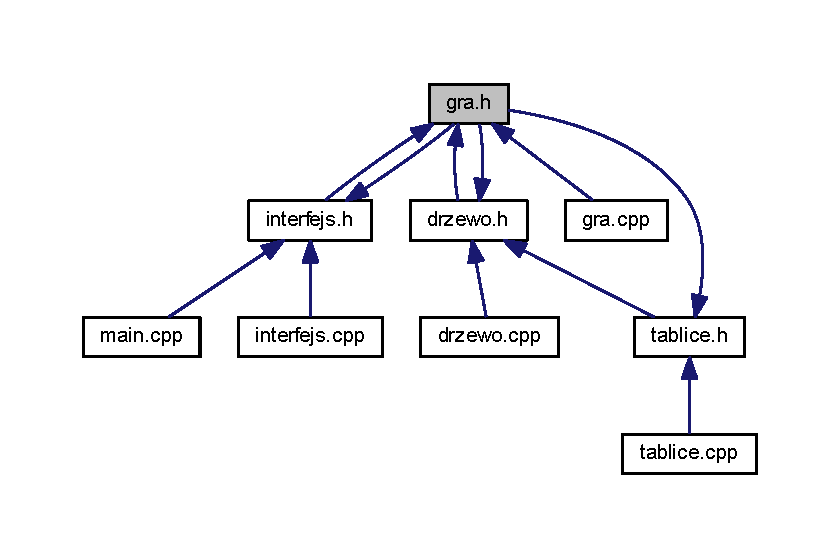
\includegraphics[width=350pt]{gra_8h__dep__incl}
\end{center}
\end{figure}
\subsection*{Komponenty}
\begin{DoxyCompactItemize}
\item 
struct \hyperlink{structosoba}{osoba}
\begin{DoxyCompactList}\small\item\em Element do wpisywania wyników. \end{DoxyCompactList}\end{DoxyCompactItemize}
\subsection*{Funkcje}
\begin{DoxyCompactItemize}
\item 
void \hyperlink{gra_8h_a472d54e5297c6dfea59903654de33ee8}{gra} ()
\begin{DoxyCompactList}\small\item\em Gra. \end{DoxyCompactList}\item 
void \hyperlink{gra_8h_ac74b2e179aafb0d5ace62ae1912cdb70}{wpisz\+\_\+tab} (char T\mbox{[}3\mbox{]}\mbox{[}3\mbox{]}, int n, char znak)
\begin{DoxyCompactList}\small\item\em Wpisywanie ruchu do planszy. \end{DoxyCompactList}\item 
int \hyperlink{gra_8h_a23182285f4fd1e760bdf5d29101488a1}{wygrana} (char T\mbox{[}3\mbox{]}\mbox{[}3\mbox{]})
\begin{DoxyCompactList}\small\item\em Sprawdzanie sytuacji. \end{DoxyCompactList}\item 
void \hyperlink{gra_8h_ae9feff07994880d9f0164bbad6aff388}{wpisz\+\_\+do\+\_\+wyniki} (int l, string nowe)
\begin{DoxyCompactList}\small\item\em Wpisywanie do wyników. \end{DoxyCompactList}\item 
void \hyperlink{gra_8h_ab0797c12c305cbec795147e947ec1e39}{nowa\+\_\+plansza} (char T\mbox{[}3\mbox{]}\mbox{[}3\mbox{]})
\begin{DoxyCompactList}\small\item\em Nowa plansza. \end{DoxyCompactList}\end{DoxyCompactItemize}


\subsection{Opis szczegółowy}
Plik nagłówkowy modułu gra. 



\subsection{Dokumentacja funkcji}
\index{gra.\+h@{gra.\+h}!gra@{gra}}
\index{gra@{gra}!gra.\+h@{gra.\+h}}
\subsubsection[{\texorpdfstring{gra()}{gra()}}]{\setlength{\rightskip}{0pt plus 5cm}void gra (
\begin{DoxyParamCaption}
{}
\end{DoxyParamCaption}
)}\hypertarget{gra_8h_a472d54e5297c6dfea59903654de33ee8}{}\label{gra_8h_a472d54e5297c6dfea59903654de33ee8}


Gra. 

Procedura przeprowadzająca grę. \index{gra.\+h@{gra.\+h}!nowa\+\_\+plansza@{nowa\+\_\+plansza}}
\index{nowa\+\_\+plansza@{nowa\+\_\+plansza}!gra.\+h@{gra.\+h}}
\subsubsection[{\texorpdfstring{nowa\+\_\+plansza(char T[3][3])}{nowa_plansza(char T[3][3])}}]{\setlength{\rightskip}{0pt plus 5cm}void nowa\+\_\+plansza (
\begin{DoxyParamCaption}
\item[{char}]{T\mbox{[}3\mbox{]}\mbox{[}3\mbox{]}}
\end{DoxyParamCaption}
)}\hypertarget{gra_8h_ab0797c12c305cbec795147e947ec1e39}{}\label{gra_8h_ab0797c12c305cbec795147e947ec1e39}


Nowa plansza. 

Procedura wypełniająca planszę znakami \textquotesingle{}-\/\textquotesingle{}. 
\begin{DoxyParams}{Parametry}
{\em T} & plansza \\
\hline
\end{DoxyParams}
\index{gra.\+h@{gra.\+h}!wpisz\+\_\+do\+\_\+wyniki@{wpisz\+\_\+do\+\_\+wyniki}}
\index{wpisz\+\_\+do\+\_\+wyniki@{wpisz\+\_\+do\+\_\+wyniki}!gra.\+h@{gra.\+h}}
\subsubsection[{\texorpdfstring{wpisz\+\_\+do\+\_\+wyniki(int l, string nowe)}{wpisz_do_wyniki(int l, string nowe)}}]{\setlength{\rightskip}{0pt plus 5cm}void wpisz\+\_\+do\+\_\+wyniki (
\begin{DoxyParamCaption}
\item[{int}]{l, }
\item[{string}]{nowe}
\end{DoxyParamCaption}
)}\hypertarget{gra_8h_ae9feff07994880d9f0164bbad6aff388}{}\label{gra_8h_ae9feff07994880d9f0164bbad6aff388}


Wpisywanie do wyników. 

Procedura dopisująca wyniku do pliku \char`\"{}wyniki.\+txt\char`\"{}. 
\begin{DoxyParams}{Parametry}
{\em l} & parametr mówiący czy dopisać wygraną(l=1), czy remis(l=0). \\
\hline
{\em nowe} & nowa nazwa gracza \\
\hline
\end{DoxyParams}
\index{gra.\+h@{gra.\+h}!wpisz\+\_\+tab@{wpisz\+\_\+tab}}
\index{wpisz\+\_\+tab@{wpisz\+\_\+tab}!gra.\+h@{gra.\+h}}
\subsubsection[{\texorpdfstring{wpisz\+\_\+tab(char T[3][3], int n, char znak)}{wpisz_tab(char T[3][3], int n, char znak)}}]{\setlength{\rightskip}{0pt plus 5cm}void wpisz\+\_\+tab (
\begin{DoxyParamCaption}
\item[{char}]{T\mbox{[}3\mbox{]}\mbox{[}3\mbox{]}, }
\item[{int}]{n, }
\item[{char}]{znak}
\end{DoxyParamCaption}
)}\hypertarget{gra_8h_ac74b2e179aafb0d5ace62ae1912cdb70}{}\label{gra_8h_ac74b2e179aafb0d5ace62ae1912cdb70}


Wpisywanie ruchu do planszy. 

Procedura wpisująca dany znak do n-\/tego wolnego miejsca na planszy T. 
\begin{DoxyParams}{Parametry}
{\em T} & plansza \\
\hline
{\em n} & numer ruchu \\
\hline
{\em znak} & znak do wpisania \\
\hline
\end{DoxyParams}
\index{gra.\+h@{gra.\+h}!wygrana@{wygrana}}
\index{wygrana@{wygrana}!gra.\+h@{gra.\+h}}
\subsubsection[{\texorpdfstring{wygrana(char T[3][3])}{wygrana(char T[3][3])}}]{\setlength{\rightskip}{0pt plus 5cm}int wygrana (
\begin{DoxyParamCaption}
\item[{char}]{T\mbox{[}3\mbox{]}\mbox{[}3\mbox{]}}
\end{DoxyParamCaption}
)}\hypertarget{gra_8h_a23182285f4fd1e760bdf5d29101488a1}{}\label{gra_8h_a23182285f4fd1e760bdf5d29101488a1}


Sprawdzanie sytuacji. 

Funkcja zwracająca w jakiej sytuacji znajduje się plansza. Zwraca 0-\/nieroztrzygnięta 1-\/wygrana kółka 2-\/wygrana krzyżyka 3-\/remis 
\begin{DoxyParams}{Parametry}
{\em T} & plansza \\
\hline
\end{DoxyParams}
\begin{DoxyReturn}{Zwraca}
sytuacja 
\end{DoxyReturn}

\hypertarget{interfejs_8cpp}{}\section{Dokumentacja pliku interfejs.\+cpp}
\label{interfejs_8cpp}\index{interfejs.\+cpp@{interfejs.\+cpp}}


Plik źródłowy modułu interfejs.  


{\ttfamily \#include \char`\"{}interfejs.\+h\char`\"{}}\\*
Wykres zależności załączania dla interfejs.\+cpp\+:\nopagebreak
\begin{figure}[H]
\begin{center}
\leavevmode
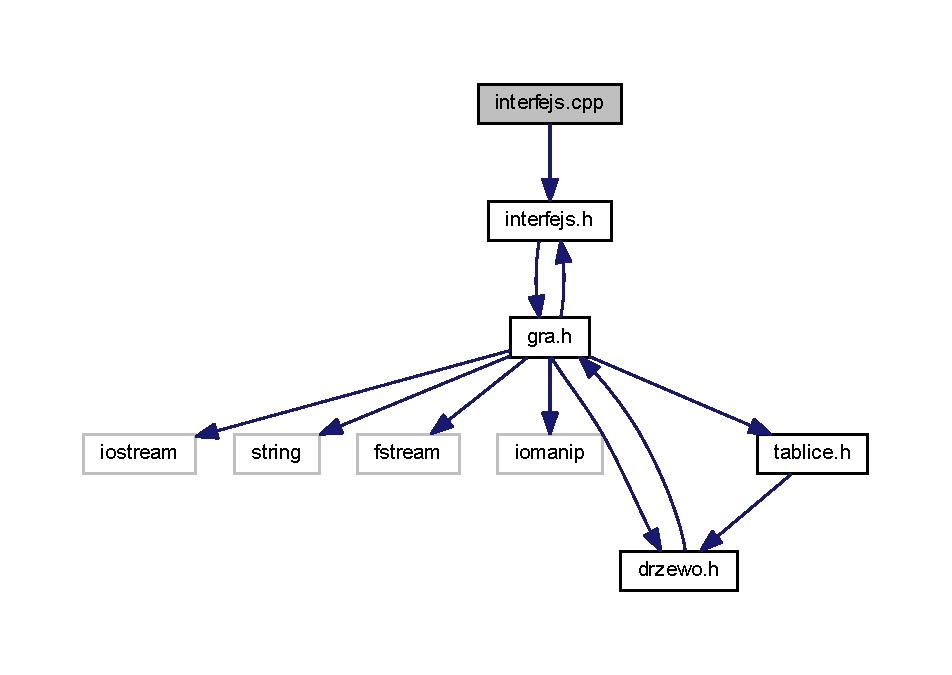
\includegraphics[width=350pt]{interfejs_8cpp__incl}
\end{center}
\end{figure}
\subsection*{Funkcje}
\begin{DoxyCompactItemize}
\item 
int \hyperlink{interfejs_8cpp_aa4419b57f1f3030c2a8dd7bab654fc66}{wczytaj\+\_\+int} ()
\begin{DoxyCompactList}\small\item\em Wczytywanie int-\/ów. \end{DoxyCompactList}\item 
void \hyperlink{interfejs_8cpp_aa4dc24d871e1269db26b741240223884}{wyniki} ()
\begin{DoxyCompactList}\small\item\em Wypisywanie wyników. \end{DoxyCompactList}\item 
void \hyperlink{interfejs_8cpp_ad1500d677f028e366ff4d32b904fb5a9}{drukuj\+\_\+plansze} (char T\mbox{[}3\mbox{]}\mbox{[}3\mbox{]})
\begin{DoxyCompactList}\small\item\em Wypisanie planszy. \end{DoxyCompactList}\item 
int \hyperlink{interfejs_8cpp_a01a8e63a894140df95ee846e79ef4db0}{podaj\+\_\+ruch} ()
\begin{DoxyCompactList}\small\item\em Wczytywanie ruchu. \end{DoxyCompactList}\item 
char \hyperlink{interfejs_8cpp_a7ae139e3cd444aebab5a4b79bd8d54e0}{wybierz\+\_\+znak} ()
\begin{DoxyCompactList}\small\item\em Wczytywanie od gracza wyboru znaku. \end{DoxyCompactList}\item 
int \hyperlink{interfejs_8cpp_a3f0496d09778c87c97169b32710d7609}{zaczyna} ()
\begin{DoxyCompactList}\small\item\em Wczytywanie od gracza kto zaczyna. \end{DoxyCompactList}\item 
string \hyperlink{interfejs_8cpp_ab7f8136fe0872e52d8d2c585f5f0676b}{podaj\+\_\+nazwe} ()
\begin{DoxyCompactList}\small\item\em Wczytywanie nazwy. \end{DoxyCompactList}\end{DoxyCompactItemize}


\subsection{Opis szczegółowy}
Plik źródłowy modułu interfejs. 



\subsection{Dokumentacja funkcji}
\index{interfejs.\+cpp@{interfejs.\+cpp}!drukuj\+\_\+plansze@{drukuj\+\_\+plansze}}
\index{drukuj\+\_\+plansze@{drukuj\+\_\+plansze}!interfejs.\+cpp@{interfejs.\+cpp}}
\subsubsection[{\texorpdfstring{drukuj\+\_\+plansze(char T[3][3])}{drukuj_plansze(char T[3][3])}}]{\setlength{\rightskip}{0pt plus 5cm}void drukuj\+\_\+plansze (
\begin{DoxyParamCaption}
\item[{char}]{T\mbox{[}3\mbox{]}\mbox{[}3\mbox{]}}
\end{DoxyParamCaption}
)}\hypertarget{interfejs_8cpp_ad1500d677f028e366ff4d32b904fb5a9}{}\label{interfejs_8cpp_ad1500d677f028e366ff4d32b904fb5a9}


Wypisanie planszy. 

Procedura wypisująca planszę. 
\begin{DoxyParams}{Parametry}
{\em T} & plansza \\
\hline
\end{DoxyParams}
\index{interfejs.\+cpp@{interfejs.\+cpp}!podaj\+\_\+nazwe@{podaj\+\_\+nazwe}}
\index{podaj\+\_\+nazwe@{podaj\+\_\+nazwe}!interfejs.\+cpp@{interfejs.\+cpp}}
\subsubsection[{\texorpdfstring{podaj\+\_\+nazwe()}{podaj_nazwe()}}]{\setlength{\rightskip}{0pt plus 5cm}string podaj\+\_\+nazwe (
\begin{DoxyParamCaption}
{}
\end{DoxyParamCaption}
)}\hypertarget{interfejs_8cpp_ab7f8136fe0872e52d8d2c585f5f0676b}{}\label{interfejs_8cpp_ab7f8136fe0872e52d8d2c585f5f0676b}


Wczytywanie nazwy. 

Funkcja interfejsu, wczytujaca od użytkownika jego nazwę do dopisania go do tablicy wyników. \begin{DoxyReturn}{Zwraca}
wczytana nazwa 
\end{DoxyReturn}
\index{interfejs.\+cpp@{interfejs.\+cpp}!podaj\+\_\+ruch@{podaj\+\_\+ruch}}
\index{podaj\+\_\+ruch@{podaj\+\_\+ruch}!interfejs.\+cpp@{interfejs.\+cpp}}
\subsubsection[{\texorpdfstring{podaj\+\_\+ruch()}{podaj_ruch()}}]{\setlength{\rightskip}{0pt plus 5cm}int podaj\+\_\+ruch (
\begin{DoxyParamCaption}
{}
\end{DoxyParamCaption}
)}\hypertarget{interfejs_8cpp_a01a8e63a894140df95ee846e79ef4db0}{}\label{interfejs_8cpp_a01a8e63a894140df95ee846e79ef4db0}


Wczytywanie ruchu. 

Funkcja wczytująca od użytkownika numer ruchu. \begin{DoxyReturn}{Zwraca}
numer ruchu 
\end{DoxyReturn}
\index{interfejs.\+cpp@{interfejs.\+cpp}!wczytaj\+\_\+int@{wczytaj\+\_\+int}}
\index{wczytaj\+\_\+int@{wczytaj\+\_\+int}!interfejs.\+cpp@{interfejs.\+cpp}}
\subsubsection[{\texorpdfstring{wczytaj\+\_\+int()}{wczytaj_int()}}]{\setlength{\rightskip}{0pt plus 5cm}int wczytaj\+\_\+int (
\begin{DoxyParamCaption}
{}
\end{DoxyParamCaption}
)}\hypertarget{interfejs_8cpp_aa4419b57f1f3030c2a8dd7bab654fc66}{}\label{interfejs_8cpp_aa4419b57f1f3030c2a8dd7bab654fc66}


Wczytywanie int-\/ów. 

Funkcja wczytujaca od użytkownika zmienną typu int. \begin{DoxyReturn}{Zwraca}
wczytany int 
\end{DoxyReturn}
\index{interfejs.\+cpp@{interfejs.\+cpp}!wybierz\+\_\+znak@{wybierz\+\_\+znak}}
\index{wybierz\+\_\+znak@{wybierz\+\_\+znak}!interfejs.\+cpp@{interfejs.\+cpp}}
\subsubsection[{\texorpdfstring{wybierz\+\_\+znak()}{wybierz_znak()}}]{\setlength{\rightskip}{0pt plus 5cm}char wybierz\+\_\+znak (
\begin{DoxyParamCaption}
{}
\end{DoxyParamCaption}
)}\hypertarget{interfejs_8cpp_a7ae139e3cd444aebab5a4b79bd8d54e0}{}\label{interfejs_8cpp_a7ae139e3cd444aebab5a4b79bd8d54e0}


Wczytywanie od gracza wyboru znaku. 

Funkcja interfejsu, wczytujaca od użytkownika numer oznaczajązy jego wybór dotyczący tego jakim znakiem będzie grał. \begin{DoxyReturn}{Zwraca}
wybrany znak 
\end{DoxyReturn}
\index{interfejs.\+cpp@{interfejs.\+cpp}!wyniki@{wyniki}}
\index{wyniki@{wyniki}!interfejs.\+cpp@{interfejs.\+cpp}}
\subsubsection[{\texorpdfstring{wyniki()}{wyniki()}}]{\setlength{\rightskip}{0pt plus 5cm}void wyniki (
\begin{DoxyParamCaption}
{}
\end{DoxyParamCaption}
)}\hypertarget{interfejs_8cpp_aa4dc24d871e1269db26b741240223884}{}\label{interfejs_8cpp_aa4dc24d871e1269db26b741240223884}


Wypisywanie wyników. 

Procedura wypisująca tablicę wyników z pliku \char`\"{}wyniki.\+txt\char`\"{}. \index{interfejs.\+cpp@{interfejs.\+cpp}!zaczyna@{zaczyna}}
\index{zaczyna@{zaczyna}!interfejs.\+cpp@{interfejs.\+cpp}}
\subsubsection[{\texorpdfstring{zaczyna()}{zaczyna()}}]{\setlength{\rightskip}{0pt plus 5cm}int zaczyna (
\begin{DoxyParamCaption}
{}
\end{DoxyParamCaption}
)}\hypertarget{interfejs_8cpp_a3f0496d09778c87c97169b32710d7609}{}\label{interfejs_8cpp_a3f0496d09778c87c97169b32710d7609}


Wczytywanie od gracza kto zaczyna. 

Funkcja interfejsu, wczytujaca od użytkownika numer oznaczajązy jego wybór dotyczący tego kto zacznie grę. \begin{DoxyReturn}{Zwraca}
wczytany numer 
\end{DoxyReturn}

\hypertarget{interfejs_8h}{}\section{Dokumentacja pliku interfejs.\+h}
\label{interfejs_8h}\index{interfejs.\+h@{interfejs.\+h}}


Plik nagłówkowy modułu interfejs.  


{\ttfamily \#include \char`\"{}gra.\+h\char`\"{}}\\*
Wykres zależności załączania dla interfejs.\+h\+:\nopagebreak
\begin{figure}[H]
\begin{center}
\leavevmode
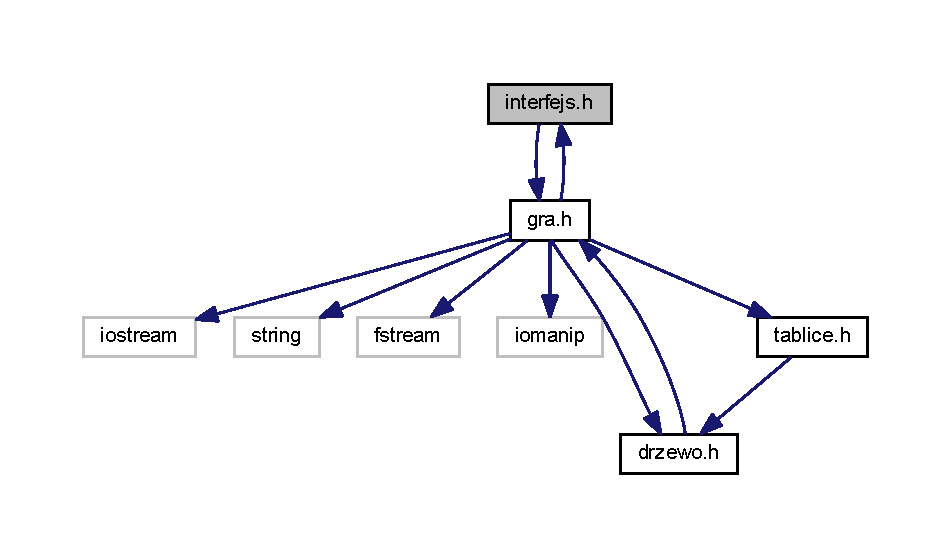
\includegraphics[width=350pt]{interfejs_8h__incl}
\end{center}
\end{figure}
Ten wykres pokazuje, które pliki bezpośrednio lub pośrednio załączają ten plik\+:\nopagebreak
\begin{figure}[H]
\begin{center}
\leavevmode
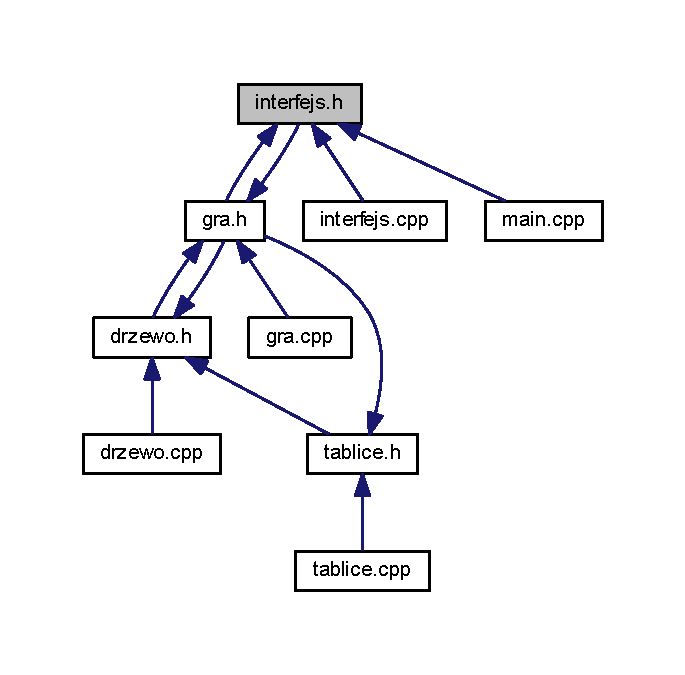
\includegraphics[width=329pt]{interfejs_8h__dep__incl}
\end{center}
\end{figure}
\subsection*{Funkcje}
\begin{DoxyCompactItemize}
\item 
int \hyperlink{interfejs_8h_aa4419b57f1f3030c2a8dd7bab654fc66}{wczytaj\+\_\+int} ()
\begin{DoxyCompactList}\small\item\em Wczytywanie int-\/ów. \end{DoxyCompactList}\item 
void \hyperlink{interfejs_8h_aa4dc24d871e1269db26b741240223884}{wyniki} ()
\begin{DoxyCompactList}\small\item\em Wypisywanie wyników. \end{DoxyCompactList}\item 
void \hyperlink{interfejs_8h_ad1500d677f028e366ff4d32b904fb5a9}{drukuj\+\_\+plansze} (char T\mbox{[}3\mbox{]}\mbox{[}3\mbox{]})
\begin{DoxyCompactList}\small\item\em Wypisanie planszy. \end{DoxyCompactList}\item 
int \hyperlink{interfejs_8h_a01a8e63a894140df95ee846e79ef4db0}{podaj\+\_\+ruch} ()
\begin{DoxyCompactList}\small\item\em Wczytywanie ruchu. \end{DoxyCompactList}\item 
char \hyperlink{interfejs_8h_a7ae139e3cd444aebab5a4b79bd8d54e0}{wybierz\+\_\+znak} ()
\begin{DoxyCompactList}\small\item\em Wczytywanie od gracza wyboru znaku. \end{DoxyCompactList}\item 
int \hyperlink{interfejs_8h_a3f0496d09778c87c97169b32710d7609}{zaczyna} ()
\begin{DoxyCompactList}\small\item\em Wczytywanie od gracza kto zaczyna. \end{DoxyCompactList}\item 
string \hyperlink{interfejs_8h_ab7f8136fe0872e52d8d2c585f5f0676b}{podaj\+\_\+nazwe} ()
\begin{DoxyCompactList}\small\item\em Wczytywanie nazwy. \end{DoxyCompactList}\end{DoxyCompactItemize}


\subsection{Opis szczegółowy}
Plik nagłówkowy modułu interfejs. 



\subsection{Dokumentacja funkcji}
\index{interfejs.\+h@{interfejs.\+h}!drukuj\+\_\+plansze@{drukuj\+\_\+plansze}}
\index{drukuj\+\_\+plansze@{drukuj\+\_\+plansze}!interfejs.\+h@{interfejs.\+h}}
\subsubsection[{\texorpdfstring{drukuj\+\_\+plansze(char T[3][3])}{drukuj_plansze(char T[3][3])}}]{\setlength{\rightskip}{0pt plus 5cm}void drukuj\+\_\+plansze (
\begin{DoxyParamCaption}
\item[{char}]{T\mbox{[}3\mbox{]}\mbox{[}3\mbox{]}}
\end{DoxyParamCaption}
)}\hypertarget{interfejs_8h_ad1500d677f028e366ff4d32b904fb5a9}{}\label{interfejs_8h_ad1500d677f028e366ff4d32b904fb5a9}


Wypisanie planszy. 

Procedura wypisująca planszę. 
\begin{DoxyParams}{Parametry}
{\em T} & plansza \\
\hline
\end{DoxyParams}
\index{interfejs.\+h@{interfejs.\+h}!podaj\+\_\+nazwe@{podaj\+\_\+nazwe}}
\index{podaj\+\_\+nazwe@{podaj\+\_\+nazwe}!interfejs.\+h@{interfejs.\+h}}
\subsubsection[{\texorpdfstring{podaj\+\_\+nazwe()}{podaj_nazwe()}}]{\setlength{\rightskip}{0pt plus 5cm}string podaj\+\_\+nazwe (
\begin{DoxyParamCaption}
{}
\end{DoxyParamCaption}
)}\hypertarget{interfejs_8h_ab7f8136fe0872e52d8d2c585f5f0676b}{}\label{interfejs_8h_ab7f8136fe0872e52d8d2c585f5f0676b}


Wczytywanie nazwy. 

Funkcja interfejsu, wczytujaca od użytkownika jego nazwę do dopisania go do tablicy wyników. \begin{DoxyReturn}{Zwraca}
wczytana nazwa 
\end{DoxyReturn}
\index{interfejs.\+h@{interfejs.\+h}!podaj\+\_\+ruch@{podaj\+\_\+ruch}}
\index{podaj\+\_\+ruch@{podaj\+\_\+ruch}!interfejs.\+h@{interfejs.\+h}}
\subsubsection[{\texorpdfstring{podaj\+\_\+ruch()}{podaj_ruch()}}]{\setlength{\rightskip}{0pt plus 5cm}int podaj\+\_\+ruch (
\begin{DoxyParamCaption}
{}
\end{DoxyParamCaption}
)}\hypertarget{interfejs_8h_a01a8e63a894140df95ee846e79ef4db0}{}\label{interfejs_8h_a01a8e63a894140df95ee846e79ef4db0}


Wczytywanie ruchu. 

Funkcja wczytująca od użytkownika numer ruchu. \begin{DoxyReturn}{Zwraca}
numer ruchu 
\end{DoxyReturn}
\index{interfejs.\+h@{interfejs.\+h}!wczytaj\+\_\+int@{wczytaj\+\_\+int}}
\index{wczytaj\+\_\+int@{wczytaj\+\_\+int}!interfejs.\+h@{interfejs.\+h}}
\subsubsection[{\texorpdfstring{wczytaj\+\_\+int()}{wczytaj_int()}}]{\setlength{\rightskip}{0pt plus 5cm}int wczytaj\+\_\+int (
\begin{DoxyParamCaption}
{}
\end{DoxyParamCaption}
)}\hypertarget{interfejs_8h_aa4419b57f1f3030c2a8dd7bab654fc66}{}\label{interfejs_8h_aa4419b57f1f3030c2a8dd7bab654fc66}


Wczytywanie int-\/ów. 

Funkcja wczytujaca od użytkownika zmienną typu int. \begin{DoxyReturn}{Zwraca}
wczytany int 
\end{DoxyReturn}
\index{interfejs.\+h@{interfejs.\+h}!wybierz\+\_\+znak@{wybierz\+\_\+znak}}
\index{wybierz\+\_\+znak@{wybierz\+\_\+znak}!interfejs.\+h@{interfejs.\+h}}
\subsubsection[{\texorpdfstring{wybierz\+\_\+znak()}{wybierz_znak()}}]{\setlength{\rightskip}{0pt plus 5cm}char wybierz\+\_\+znak (
\begin{DoxyParamCaption}
{}
\end{DoxyParamCaption}
)}\hypertarget{interfejs_8h_a7ae139e3cd444aebab5a4b79bd8d54e0}{}\label{interfejs_8h_a7ae139e3cd444aebab5a4b79bd8d54e0}


Wczytywanie od gracza wyboru znaku. 

Funkcja interfejsu, wczytujaca od użytkownika numer oznaczajązy jego wybór dotyczący tego jakim znakiem będzie grał. \begin{DoxyReturn}{Zwraca}
wybrany znak 
\end{DoxyReturn}
\index{interfejs.\+h@{interfejs.\+h}!wyniki@{wyniki}}
\index{wyniki@{wyniki}!interfejs.\+h@{interfejs.\+h}}
\subsubsection[{\texorpdfstring{wyniki()}{wyniki()}}]{\setlength{\rightskip}{0pt plus 5cm}void wyniki (
\begin{DoxyParamCaption}
{}
\end{DoxyParamCaption}
)}\hypertarget{interfejs_8h_aa4dc24d871e1269db26b741240223884}{}\label{interfejs_8h_aa4dc24d871e1269db26b741240223884}


Wypisywanie wyników. 

Procedura wypisująca tablicę wyników z pliku \char`\"{}wyniki.\+txt\char`\"{}. \index{interfejs.\+h@{interfejs.\+h}!zaczyna@{zaczyna}}
\index{zaczyna@{zaczyna}!interfejs.\+h@{interfejs.\+h}}
\subsubsection[{\texorpdfstring{zaczyna()}{zaczyna()}}]{\setlength{\rightskip}{0pt plus 5cm}int zaczyna (
\begin{DoxyParamCaption}
{}
\end{DoxyParamCaption}
)}\hypertarget{interfejs_8h_a3f0496d09778c87c97169b32710d7609}{}\label{interfejs_8h_a3f0496d09778c87c97169b32710d7609}


Wczytywanie od gracza kto zaczyna. 

Funkcja interfejsu, wczytujaca od użytkownika numer oznaczajązy jego wybór dotyczący tego kto zacznie grę. \begin{DoxyReturn}{Zwraca}
wczytany numer 
\end{DoxyReturn}

\hypertarget{main_8cpp}{}\section{Dokumentacja pliku main.\+cpp}
\label{main_8cpp}\index{main.\+cpp@{main.\+cpp}}


Plik źródłowy główny.  


{\ttfamily \#include \char`\"{}interfejs.\+h\char`\"{}}\\*
Wykres zależności załączania dla main.\+cpp\+:\nopagebreak
\begin{figure}[H]
\begin{center}
\leavevmode
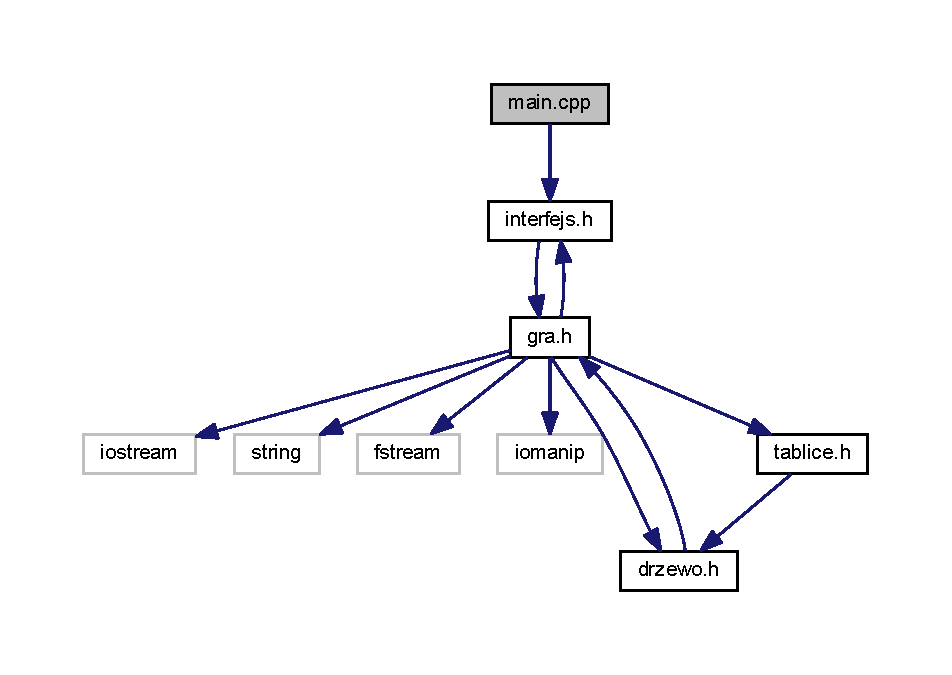
\includegraphics[width=350pt]{main_8cpp__incl}
\end{center}
\end{figure}
\subsection*{Funkcje}
\begin{DoxyCompactItemize}
\item 
int \hyperlink{main_8cpp_ae66f6b31b5ad750f1fe042a706a4e3d4}{main} ()
\end{DoxyCompactItemize}


\subsection{Opis szczegółowy}
Plik źródłowy główny. 



\subsection{Dokumentacja funkcji}
\index{main.\+cpp@{main.\+cpp}!main@{main}}
\index{main@{main}!main.\+cpp@{main.\+cpp}}
\subsubsection[{\texorpdfstring{main()}{main()}}]{\setlength{\rightskip}{0pt plus 5cm}int main (
\begin{DoxyParamCaption}
{}
\end{DoxyParamCaption}
)}\hypertarget{main_8cpp_ae66f6b31b5ad750f1fe042a706a4e3d4}{}\label{main_8cpp_ae66f6b31b5ad750f1fe042a706a4e3d4}

\hypertarget{tablice_8cpp}{}\section{Dokumentacja pliku tablice.\+cpp}
\label{tablice_8cpp}\index{tablice.\+cpp@{tablice.\+cpp}}


Plik źródłowy modułu tablice.  


{\ttfamily \#include \char`\"{}tablice.\+h\char`\"{}}\\*
Wykres zależności załączania dla tablice.\+cpp\+:\nopagebreak
\begin{figure}[H]
\begin{center}
\leavevmode
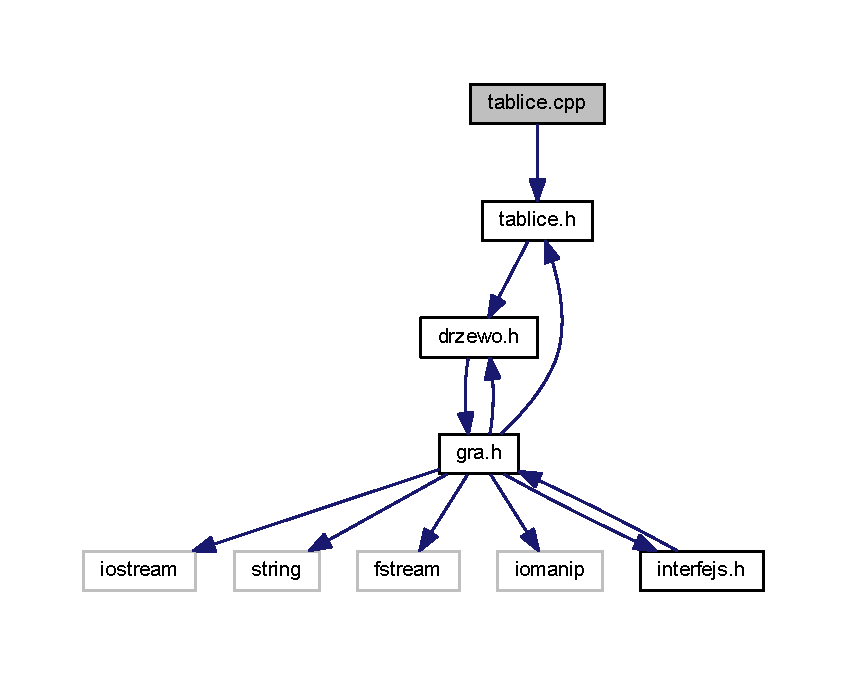
\includegraphics[width=350pt]{tablice_8cpp__incl}
\end{center}
\end{figure}
\subsection*{Funkcje}
\begin{DoxyCompactItemize}
\item 
void \hyperlink{tablice_8cpp_a97ef69276f5e27f59c6cb1da7f311ced}{lista\+\_\+tab} (\hyperlink{structtab}{tab} $\ast$\&t, int N, \hyperlink{structwezel}{wezel} $\ast$pop, int licznik, int nr)
\begin{DoxyCompactList}\small\item\em Tworzenie listy. \end{DoxyCompactList}\item 
void \hyperlink{tablice_8cpp_a06b2e02c3511e4acd25ccd5f26ed9dbe}{usun\+\_\+tab} (\hyperlink{structtab}{tab} $\ast$\&k)
\begin{DoxyCompactList}\small\item\em Usuwanie listy. \end{DoxyCompactList}\item 
int $\ast$ \hyperlink{tablice_8cpp_a820a840ec301f638919a2e1917640a7d}{nowa\+\_\+tab} (int N)
\begin{DoxyCompactList}\small\item\em Tworzenie nowej tablicy. \end{DoxyCompactList}\item 
int \hyperlink{tablice_8cpp_a06f35e1bc01e5e6414fbbcb9895375f2}{ruch\+\_\+komp} (\hyperlink{structtab}{tab} $\ast$t, int N)
\begin{DoxyCompactList}\small\item\em Wybór ruchu komputera. \end{DoxyCompactList}\item 
bool \hyperlink{tablice_8cpp_a545123090d1b2cde9850d53ae29f3dd7}{czy\+\_\+pelna\+\_\+tab} (int $\ast$T, int N)
\begin{DoxyCompactList}\small\item\em Sprawdznie czy tablica jest pełna. \end{DoxyCompactList}\item 
bool \hyperlink{tablice_8cpp_a6e5296e1097e256322d15ed95f6048b2}{czy\+\_\+prawie\+\_\+pelna\+\_\+tab} (int $\ast$T, int N)
\begin{DoxyCompactList}\small\item\em Sprawdznie czy tablica jest prawie pełna. \end{DoxyCompactList}\end{DoxyCompactItemize}


\subsection{Opis szczegółowy}
Plik źródłowy modułu tablice. 



\subsection{Dokumentacja funkcji}
\index{tablice.\+cpp@{tablice.\+cpp}!czy\+\_\+pelna\+\_\+tab@{czy\+\_\+pelna\+\_\+tab}}
\index{czy\+\_\+pelna\+\_\+tab@{czy\+\_\+pelna\+\_\+tab}!tablice.\+cpp@{tablice.\+cpp}}
\subsubsection[{\texorpdfstring{czy\+\_\+pelna\+\_\+tab(int $\ast$\+T, int N)}{czy_pelna_tab(int *T, int N)}}]{\setlength{\rightskip}{0pt plus 5cm}bool czy\+\_\+pelna\+\_\+tab (
\begin{DoxyParamCaption}
\item[{int $\ast$}]{T, }
\item[{int}]{N}
\end{DoxyParamCaption}
)}\hypertarget{tablice_8cpp_a545123090d1b2cde9850d53ae29f3dd7}{}\label{tablice_8cpp_a545123090d1b2cde9850d53ae29f3dd7}


Sprawdznie czy tablica jest pełna. 

Funkcja sprawdzająca czy dana tablica T ma jakieś pole równe 0, wówczas zwracająca false. 
\begin{DoxyParams}{Parametry}
{\em T} & wskaźnik tablicy \\
\hline
{\em N} & wielkość tablicy \\
\hline
\end{DoxyParams}
\begin{DoxyReturn}{Zwraca}
czy tablica jest pełna 
\end{DoxyReturn}
\index{tablice.\+cpp@{tablice.\+cpp}!czy\+\_\+prawie\+\_\+pelna\+\_\+tab@{czy\+\_\+prawie\+\_\+pelna\+\_\+tab}}
\index{czy\+\_\+prawie\+\_\+pelna\+\_\+tab@{czy\+\_\+prawie\+\_\+pelna\+\_\+tab}!tablice.\+cpp@{tablice.\+cpp}}
\subsubsection[{\texorpdfstring{czy\+\_\+prawie\+\_\+pelna\+\_\+tab(int $\ast$\+T, int N)}{czy_prawie_pelna_tab(int *T, int N)}}]{\setlength{\rightskip}{0pt plus 5cm}bool czy\+\_\+prawie\+\_\+pelna\+\_\+tab (
\begin{DoxyParamCaption}
\item[{int $\ast$}]{T, }
\item[{int}]{N}
\end{DoxyParamCaption}
)}\hypertarget{tablice_8cpp_a6e5296e1097e256322d15ed95f6048b2}{}\label{tablice_8cpp_a6e5296e1097e256322d15ed95f6048b2}


Sprawdznie czy tablica jest prawie pełna. 

Funkcja sprawdzająca czy dana tablica T ma dokładnie jedno pole równe 0, wówczas zwracająca true. 
\begin{DoxyParams}{Parametry}
{\em T} & wskaźnik tablicy \\
\hline
{\em N} & wielkość tablicy \\
\hline
\end{DoxyParams}
\begin{DoxyReturn}{Zwraca}
czy tablica jest prawnie pełna 
\end{DoxyReturn}
\index{tablice.\+cpp@{tablice.\+cpp}!lista\+\_\+tab@{lista\+\_\+tab}}
\index{lista\+\_\+tab@{lista\+\_\+tab}!tablice.\+cpp@{tablice.\+cpp}}
\subsubsection[{\texorpdfstring{lista\+\_\+tab(tab $\ast$\&t, int N, wezel $\ast$pop, int licznik, int nr)}{lista_tab(tab *&t, int N, wezel *pop, int licznik, int nr)}}]{\setlength{\rightskip}{0pt plus 5cm}void lista\+\_\+tab (
\begin{DoxyParamCaption}
\item[{{\bf tab} $\ast$\&}]{t, }
\item[{int}]{N, }
\item[{{\bf wezel} $\ast$}]{pop, }
\item[{int}]{licznik, }
\item[{int}]{nr}
\end{DoxyParamCaption}
)}\hypertarget{tablice_8cpp_a97ef69276f5e27f59c6cb1da7f311ced}{}\label{tablice_8cpp_a97ef69276f5e27f59c6cb1da7f311ced}


Tworzenie listy. 

Procedura rekurencyjna tworząca nową listę tablic. 
\begin{DoxyParams}{Parametry}
{\em t} & poprzedni element listy \\
\hline
{\em N} & liczba możliwych do wykonania przez kompuer ruchów \\
\hline
{\em pop} & element drzewa, z którego zczytywane są liczby wygranych, przegranych i remisów dla następnego ruchu \\
\hline
{\em licznik} & numer określający, który to z kolei wykonywany ruch \\
\hline
{\em nr} & numer wykonywanego ruchu \\
\hline
\end{DoxyParams}
\index{tablice.\+cpp@{tablice.\+cpp}!nowa\+\_\+tab@{nowa\+\_\+tab}}
\index{nowa\+\_\+tab@{nowa\+\_\+tab}!tablice.\+cpp@{tablice.\+cpp}}
\subsubsection[{\texorpdfstring{nowa\+\_\+tab(int N)}{nowa_tab(int N)}}]{\setlength{\rightskip}{0pt plus 5cm}int$\ast$ nowa\+\_\+tab (
\begin{DoxyParamCaption}
\item[{int}]{N}
\end{DoxyParamCaption}
)}\hypertarget{tablice_8cpp_a820a840ec301f638919a2e1917640a7d}{}\label{tablice_8cpp_a820a840ec301f638919a2e1917640a7d}


Tworzenie nowej tablicy. 

Funkcja tworząca nową tablicę jednowymiarową dynamiczną o wielkości N i zwracająca jej wskaźnik. 
\begin{DoxyParams}{Parametry}
{\em N} & wielkość tablicy \\
\hline
\end{DoxyParams}
\begin{DoxyReturn}{Zwraca}
wskaźnik tablicy 
\end{DoxyReturn}
\index{tablice.\+cpp@{tablice.\+cpp}!ruch\+\_\+komp@{ruch\+\_\+komp}}
\index{ruch\+\_\+komp@{ruch\+\_\+komp}!tablice.\+cpp@{tablice.\+cpp}}
\subsubsection[{\texorpdfstring{ruch\+\_\+komp(tab $\ast$t, int N)}{ruch_komp(tab *t, int N)}}]{\setlength{\rightskip}{0pt plus 5cm}int ruch\+\_\+komp (
\begin{DoxyParamCaption}
\item[{{\bf tab} $\ast$}]{x, }
\item[{int}]{N}
\end{DoxyParamCaption}
)}\hypertarget{tablice_8cpp_a06f35e1bc01e5e6414fbbcb9895375f2}{}\label{tablice_8cpp_a06f35e1bc01e5e6414fbbcb9895375f2}


Wybór ruchu komputera. 

Funkcja zwracająca numer ruchu do wykonania dla komputera na podstawie listy tablic. 
\begin{DoxyParams}{Parametry}
{\em x} & głowa listy \\
\hline
{\em N} & liczba możliwych do wykonania ruchów \\
\hline
\end{DoxyParams}
\begin{DoxyReturn}{Zwraca}
numer ruchu 
\end{DoxyReturn}
\index{tablice.\+cpp@{tablice.\+cpp}!usun\+\_\+tab@{usun\+\_\+tab}}
\index{usun\+\_\+tab@{usun\+\_\+tab}!tablice.\+cpp@{tablice.\+cpp}}
\subsubsection[{\texorpdfstring{usun\+\_\+tab(tab $\ast$\&k)}{usun_tab(tab *&k)}}]{\setlength{\rightskip}{0pt plus 5cm}void usun\+\_\+tab (
\begin{DoxyParamCaption}
\item[{{\bf tab} $\ast$\&}]{k}
\end{DoxyParamCaption}
)}\hypertarget{tablice_8cpp_a06b2e02c3511e4acd25ccd5f26ed9dbe}{}\label{tablice_8cpp_a06b2e02c3511e4acd25ccd5f26ed9dbe}


Usuwanie listy. 

Procedura rekurencyjna usuwająca listę tablic. 
\begin{DoxyParams}{Parametry}
{\em k} & głowa listy \\
\hline
\end{DoxyParams}

\hypertarget{tablice_8h}{}\section{Dokumentacja pliku tablice.\+h}
\label{tablice_8h}\index{tablice.\+h@{tablice.\+h}}


Plik nagłówkowy modułu tablice.  


{\ttfamily \#include \char`\"{}drzewo.\+h\char`\"{}}\\*
Wykres zależności załączania dla tablice.\+h\+:\nopagebreak
\begin{figure}[H]
\begin{center}
\leavevmode
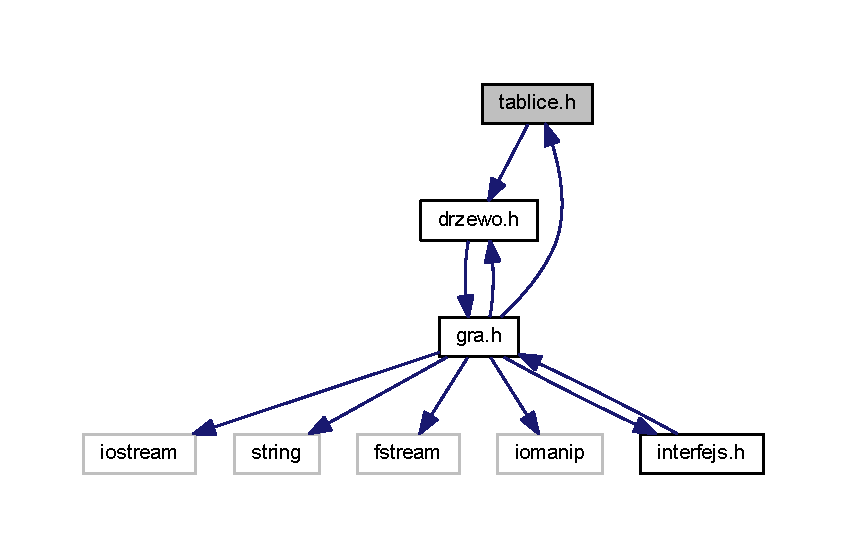
\includegraphics[width=350pt]{tablice_8h__incl}
\end{center}
\end{figure}
Ten wykres pokazuje, które pliki bezpośrednio lub pośrednio załączają ten plik\+:\nopagebreak
\begin{figure}[H]
\begin{center}
\leavevmode
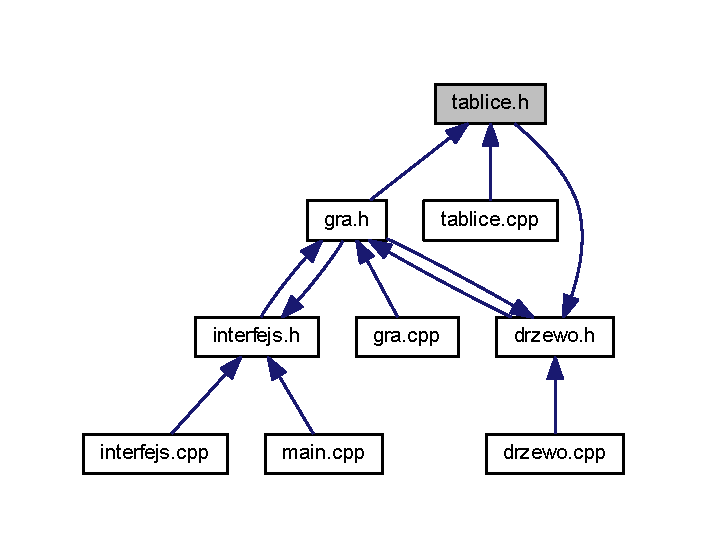
\includegraphics[width=340pt]{tablice_8h__dep__incl}
\end{center}
\end{figure}
\subsection*{Komponenty}
\begin{DoxyCompactItemize}
\item 
struct \hyperlink{structtab}{tab}
\begin{DoxyCompactList}\small\item\em Element listy dynamicznej tablic. \end{DoxyCompactList}\end{DoxyCompactItemize}
\subsection*{Funkcje}
\begin{DoxyCompactItemize}
\item 
void \hyperlink{tablice_8h_a97ef69276f5e27f59c6cb1da7f311ced}{lista\+\_\+tab} (\hyperlink{structtab}{tab} $\ast$\&t, int N, \hyperlink{structwezel}{wezel} $\ast$pop, int licznik, int nr)
\begin{DoxyCompactList}\small\item\em Tworzenie listy. \end{DoxyCompactList}\item 
void \hyperlink{tablice_8h_a06b2e02c3511e4acd25ccd5f26ed9dbe}{usun\+\_\+tab} (\hyperlink{structtab}{tab} $\ast$\&k)
\begin{DoxyCompactList}\small\item\em Usuwanie listy. \end{DoxyCompactList}\item 
int \hyperlink{tablice_8h_a1438246f4c5fc63d581202ac34f0bd1f}{ruch\+\_\+komp} (\hyperlink{structtab}{tab} $\ast$x, int N)
\begin{DoxyCompactList}\small\item\em Wybór ruchu komputera. \end{DoxyCompactList}\item 
int $\ast$ \hyperlink{tablice_8h_a820a840ec301f638919a2e1917640a7d}{nowa\+\_\+tab} (int N)
\begin{DoxyCompactList}\small\item\em Tworzenie nowej tablicy. \end{DoxyCompactList}\item 
bool \hyperlink{tablice_8h_a545123090d1b2cde9850d53ae29f3dd7}{czy\+\_\+pelna\+\_\+tab} (int $\ast$T, int N)
\begin{DoxyCompactList}\small\item\em Sprawdznie czy tablica jest pełna. \end{DoxyCompactList}\item 
bool \hyperlink{tablice_8h_a6e5296e1097e256322d15ed95f6048b2}{czy\+\_\+prawie\+\_\+pelna\+\_\+tab} (int $\ast$T, int N)
\begin{DoxyCompactList}\small\item\em Sprawdznie czy tablica jest prawie pełna. \end{DoxyCompactList}\end{DoxyCompactItemize}


\subsection{Opis szczegółowy}
Plik nagłówkowy modułu tablice. 



\subsection{Dokumentacja funkcji}
\index{tablice.\+h@{tablice.\+h}!czy\+\_\+pelna\+\_\+tab@{czy\+\_\+pelna\+\_\+tab}}
\index{czy\+\_\+pelna\+\_\+tab@{czy\+\_\+pelna\+\_\+tab}!tablice.\+h@{tablice.\+h}}
\subsubsection[{\texorpdfstring{czy\+\_\+pelna\+\_\+tab(int $\ast$\+T, int N)}{czy_pelna_tab(int *T, int N)}}]{\setlength{\rightskip}{0pt plus 5cm}bool czy\+\_\+pelna\+\_\+tab (
\begin{DoxyParamCaption}
\item[{int $\ast$}]{T, }
\item[{int}]{N}
\end{DoxyParamCaption}
)}\hypertarget{tablice_8h_a545123090d1b2cde9850d53ae29f3dd7}{}\label{tablice_8h_a545123090d1b2cde9850d53ae29f3dd7}


Sprawdznie czy tablica jest pełna. 

Funkcja sprawdzająca czy dana tablica T ma jakieś pole równe 0, wówczas zwracająca false. 
\begin{DoxyParams}{Parametry}
{\em T} & wskaźnik tablicy \\
\hline
{\em N} & wielkość tablicy \\
\hline
\end{DoxyParams}
\begin{DoxyReturn}{Zwraca}
czy tablica jest pełna 
\end{DoxyReturn}
\index{tablice.\+h@{tablice.\+h}!czy\+\_\+prawie\+\_\+pelna\+\_\+tab@{czy\+\_\+prawie\+\_\+pelna\+\_\+tab}}
\index{czy\+\_\+prawie\+\_\+pelna\+\_\+tab@{czy\+\_\+prawie\+\_\+pelna\+\_\+tab}!tablice.\+h@{tablice.\+h}}
\subsubsection[{\texorpdfstring{czy\+\_\+prawie\+\_\+pelna\+\_\+tab(int $\ast$\+T, int N)}{czy_prawie_pelna_tab(int *T, int N)}}]{\setlength{\rightskip}{0pt plus 5cm}bool czy\+\_\+prawie\+\_\+pelna\+\_\+tab (
\begin{DoxyParamCaption}
\item[{int $\ast$}]{T, }
\item[{int}]{N}
\end{DoxyParamCaption}
)}\hypertarget{tablice_8h_a6e5296e1097e256322d15ed95f6048b2}{}\label{tablice_8h_a6e5296e1097e256322d15ed95f6048b2}


Sprawdznie czy tablica jest prawie pełna. 

Funkcja sprawdzająca czy dana tablica T ma dokładnie jedno pole równe 0, wówczas zwracająca true. 
\begin{DoxyParams}{Parametry}
{\em T} & wskaźnik tablicy \\
\hline
{\em N} & wielkość tablicy \\
\hline
\end{DoxyParams}
\begin{DoxyReturn}{Zwraca}
czy tablica jest prawnie pełna 
\end{DoxyReturn}
\index{tablice.\+h@{tablice.\+h}!lista\+\_\+tab@{lista\+\_\+tab}}
\index{lista\+\_\+tab@{lista\+\_\+tab}!tablice.\+h@{tablice.\+h}}
\subsubsection[{\texorpdfstring{lista\+\_\+tab(tab $\ast$\&t, int N, wezel $\ast$pop, int licznik, int nr)}{lista_tab(tab *&t, int N, wezel *pop, int licznik, int nr)}}]{\setlength{\rightskip}{0pt plus 5cm}void lista\+\_\+tab (
\begin{DoxyParamCaption}
\item[{{\bf tab} $\ast$\&}]{t, }
\item[{int}]{N, }
\item[{{\bf wezel} $\ast$}]{pop, }
\item[{int}]{licznik, }
\item[{int}]{nr}
\end{DoxyParamCaption}
)}\hypertarget{tablice_8h_a97ef69276f5e27f59c6cb1da7f311ced}{}\label{tablice_8h_a97ef69276f5e27f59c6cb1da7f311ced}


Tworzenie listy. 

Procedura rekurencyjna tworząca nową listę tablic. 
\begin{DoxyParams}{Parametry}
{\em t} & poprzedni element listy \\
\hline
{\em N} & liczba możliwych do wykonania przez kompuer ruchów \\
\hline
{\em pop} & element drzewa, z którego zczytywane są liczby wygranych, przegranych i remisów dla następnego ruchu \\
\hline
{\em licznik} & numer określający, który to z kolei wykonywany ruch \\
\hline
{\em nr} & numer wykonywanego ruchu \\
\hline
\end{DoxyParams}
\index{tablice.\+h@{tablice.\+h}!nowa\+\_\+tab@{nowa\+\_\+tab}}
\index{nowa\+\_\+tab@{nowa\+\_\+tab}!tablice.\+h@{tablice.\+h}}
\subsubsection[{\texorpdfstring{nowa\+\_\+tab(int N)}{nowa_tab(int N)}}]{\setlength{\rightskip}{0pt plus 5cm}int$\ast$ nowa\+\_\+tab (
\begin{DoxyParamCaption}
\item[{int}]{N}
\end{DoxyParamCaption}
)}\hypertarget{tablice_8h_a820a840ec301f638919a2e1917640a7d}{}\label{tablice_8h_a820a840ec301f638919a2e1917640a7d}


Tworzenie nowej tablicy. 

Funkcja tworząca nową tablicę jednowymiarową dynamiczną o wielkości N i zwracająca jej wskaźnik. 
\begin{DoxyParams}{Parametry}
{\em N} & wielkość tablicy \\
\hline
\end{DoxyParams}
\begin{DoxyReturn}{Zwraca}
wskaźnik tablicy 
\end{DoxyReturn}
\index{tablice.\+h@{tablice.\+h}!ruch\+\_\+komp@{ruch\+\_\+komp}}
\index{ruch\+\_\+komp@{ruch\+\_\+komp}!tablice.\+h@{tablice.\+h}}
\subsubsection[{\texorpdfstring{ruch\+\_\+komp(tab $\ast$x, int N)}{ruch_komp(tab *x, int N)}}]{\setlength{\rightskip}{0pt plus 5cm}int ruch\+\_\+komp (
\begin{DoxyParamCaption}
\item[{{\bf tab} $\ast$}]{x, }
\item[{int}]{N}
\end{DoxyParamCaption}
)}\hypertarget{tablice_8h_a1438246f4c5fc63d581202ac34f0bd1f}{}\label{tablice_8h_a1438246f4c5fc63d581202ac34f0bd1f}


Wybór ruchu komputera. 

Funkcja zwracająca numer ruchu do wykonania dla komputera na podstawie listy tablic. 
\begin{DoxyParams}{Parametry}
{\em x} & głowa listy \\
\hline
{\em N} & liczba możliwych do wykonania ruchów \\
\hline
\end{DoxyParams}
\begin{DoxyReturn}{Zwraca}
numer ruchu 
\end{DoxyReturn}
\index{tablice.\+h@{tablice.\+h}!usun\+\_\+tab@{usun\+\_\+tab}}
\index{usun\+\_\+tab@{usun\+\_\+tab}!tablice.\+h@{tablice.\+h}}
\subsubsection[{\texorpdfstring{usun\+\_\+tab(tab $\ast$\&k)}{usun_tab(tab *&k)}}]{\setlength{\rightskip}{0pt plus 5cm}void usun\+\_\+tab (
\begin{DoxyParamCaption}
\item[{{\bf tab} $\ast$\&}]{k}
\end{DoxyParamCaption}
)}\hypertarget{tablice_8h_a06b2e02c3511e4acd25ccd5f26ed9dbe}{}\label{tablice_8h_a06b2e02c3511e4acd25ccd5f26ed9dbe}


Usuwanie listy. 

Procedura rekurencyjna usuwająca listę tablic. 
\begin{DoxyParams}{Parametry}
{\em k} & głowa listy \\
\hline
\end{DoxyParams}

%--- End generated contents ---

% Index
\backmatter
\newpage
\phantomsection
\clearemptydoublepage
\addcontentsline{toc}{chapter}{Indeks}
\printindex

\end{document}
